\pdfminorversion=4
\documentclass[aspectratio=169]{beamer}

\mode<presentation>
{
  \usetheme{default}
  \usecolortheme{default}
  \usefonttheme{default}
  \setbeamertemplate{navigation symbols}{}
  \setbeamertemplate{caption}[numbered]
  \setbeamertemplate{footline}[frame number]  % or "page number"
  \setbeamercolor{frametitle}{fg=white}
  \setbeamercolor{footline}{fg=black}
} 

\usepackage[english]{babel}
\usepackage[utf8x]{inputenc}
\usepackage{tikz}
\usepackage{courier}
\usepackage{array}
\usepackage{bold-extra}
\usepackage{minted}
\usepackage[thicklines]{cancel}
\usepackage{fancyvrb}

\xdefinecolor{dianablue}{rgb}{0.18,0.24,0.31}
\xdefinecolor{darkblue}{rgb}{0.1,0.1,0.7}
\xdefinecolor{darkgreen}{rgb}{0,0.5,0}
\xdefinecolor{darkgrey}{rgb}{0.35,0.35,0.35}
\xdefinecolor{darkorange}{rgb}{0.8,0.5,0}
\xdefinecolor{darkred}{rgb}{0.7,0,0}
\definecolor{darkgreen}{rgb}{0,0.6,0}
\definecolor{mauve}{rgb}{0.58,0,0.82}

\title[2022-03-09-nsf-irishep-analysis-tools]{Data Science Tools for Analysis}
\author{Jim Pivarski}
\institute{Princeton University -- IRIS-HEP}
\date{March 9, 2022}

\usetikzlibrary{shapes.callouts}

\begin{document}

\logo{\pgfputat{\pgfxy(0.11, 7.4)}{\pgfbox[right,base]{\tikz{\filldraw[fill=dianablue, draw=none] (0 cm, 0 cm) rectangle (50 cm, 1 cm);}\mbox{\hspace{-8 cm}
\includegraphics[height=1 cm]{princeton-logo-long.png}\hspace{0.1 cm}\raisebox{0.1 cm}{
\includegraphics[height=0.8 cm]{iris-hep-logo-long.png}}\hspace{0.1 cm}}}}}

\begin{frame}
  \titlepage
\end{frame}

\logo{\pgfputat{\pgfxy(0.11, 7.4)}{\pgfbox[right,base]{\tikz{\filldraw[fill=dianablue, draw=none] (0 cm, 0 cm) rectangle (50 cm, 1 cm);}\mbox{\hspace{-8 cm}
\includegraphics[height=1 cm]{princeton-logo.png}\hspace{0.1 cm}\raisebox{0.1 cm}{
\includegraphics[height=0.8 cm]{iris-hep-logo.png}}\hspace{0.1 cm}}}}}

% Uncomment these lines for an automatically generated outline.
%\begin{frame}{Outline}
%  \tableofcontents
%\end{frame}

% START START START START START START START START START START START START START

\begin{frame}{Previously (Alexander Held \& Oksana Shadura, Nov 30, 2021)}
\begin{columns}
\column{1.1\linewidth}
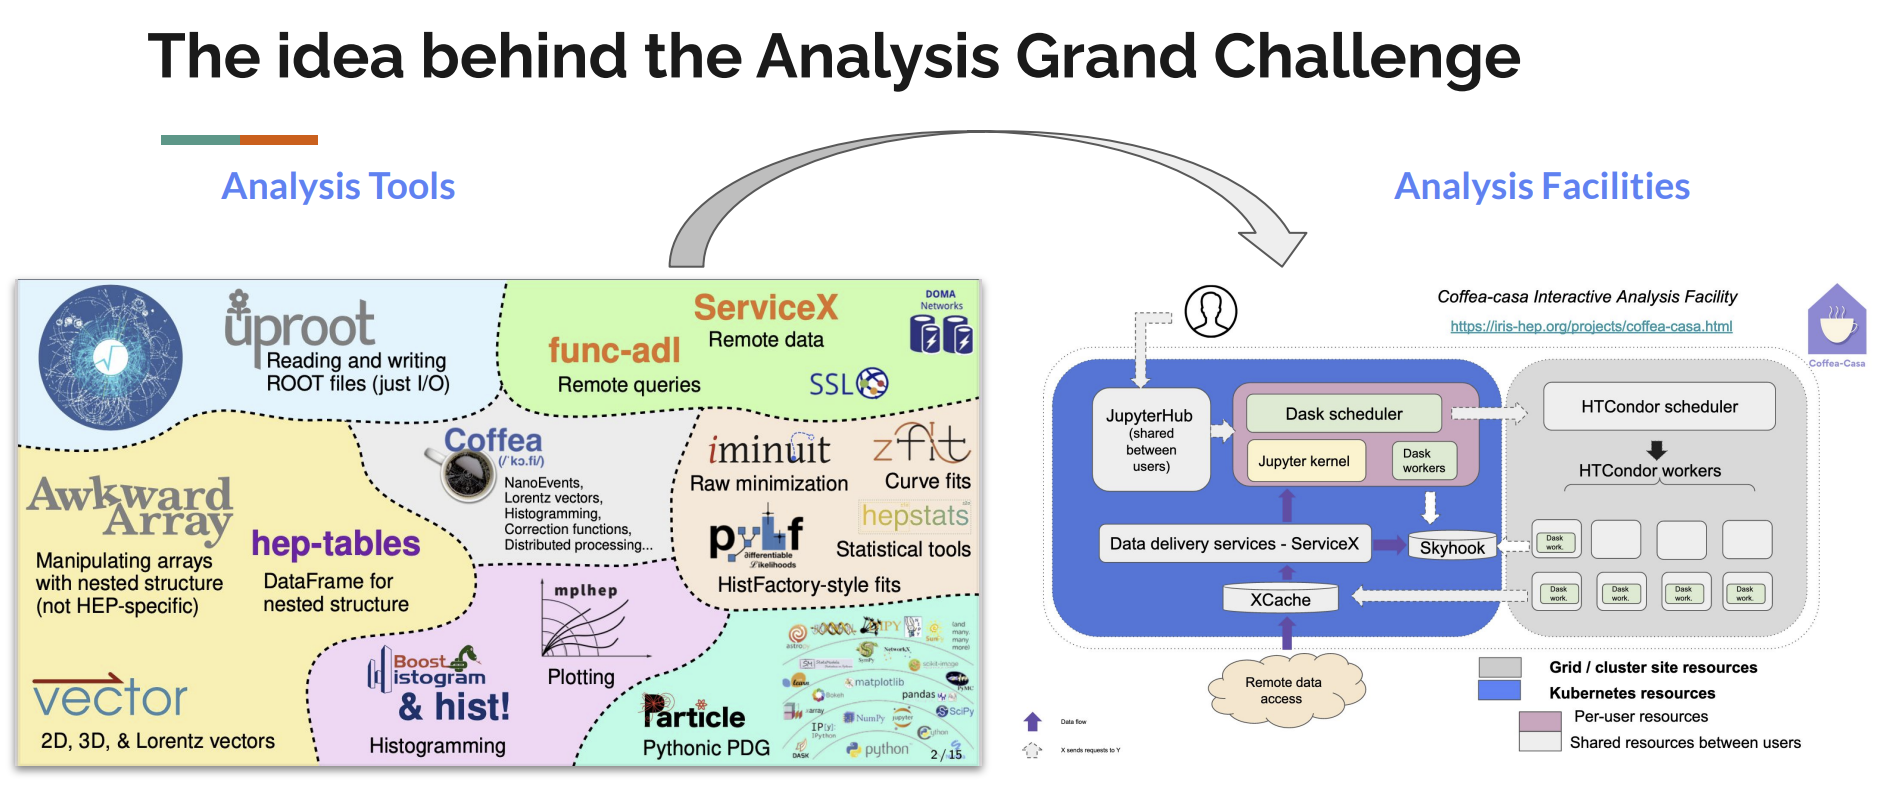
\includegraphics[width=\linewidth]{from-analysis-grand-challenge.png}
\end{columns}
\end{frame}

\begin{frame}{The analysis tools developer community}
\large
{\Large Many people are developing tools\ldots}

\vspace{0.5 cm}
\begin{itemize}\setlength{\itemsep}{0.25 cm}
\item<2-> in IRIS-HEP and out (but mostly communicating on IRIS-HEP's Slack)
\item<3-> each focused on a single purpose, but fitting together into a larger ecosystem
\item<4-> using existing software from beyond HEP whenever possible
\item<5-> mostly in Python
\end{itemize}
\end{frame}

\begin{frame}{Overview of these activities for the LHCC (\href{https://arxiv.org/abs/2202.02194}{arXiv:2202.02194})}
\vspace{0.22 cm}
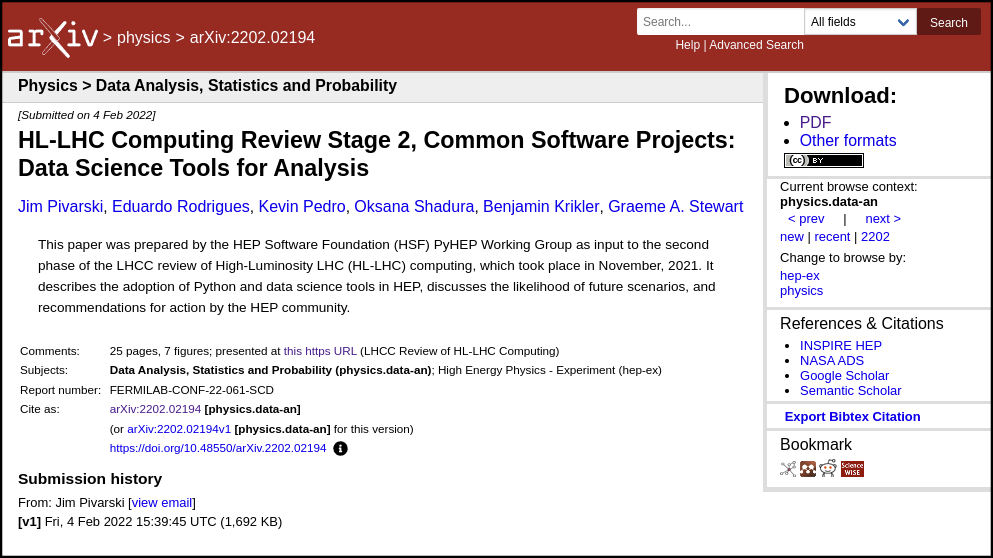
\includegraphics[width=\linewidth]{hl-lhc-data-science-tools-arXiv.png}
\end{frame}

\begin{frame}{\mbox{ }}
\begin{center}
\begin{minipage}{0.85\linewidth}
\large
{\Large A bit different from an ordinary LHC project:}

\vspace{0.25 cm}
\begin{itemize}\setlength{\itemsep}{0.25 cm}
\item The users are distributed (who are they? what do they want?)
\item The developers are distributed (who's working on what?)
\end{itemize}
\end{minipage}
\end{center}
\end{frame}

\begin{frame}{Gathered developers by lighting a beacon: Scikit-HEP}
\vspace{0.18 cm}
\begin{columns}
\column{1.15\linewidth}
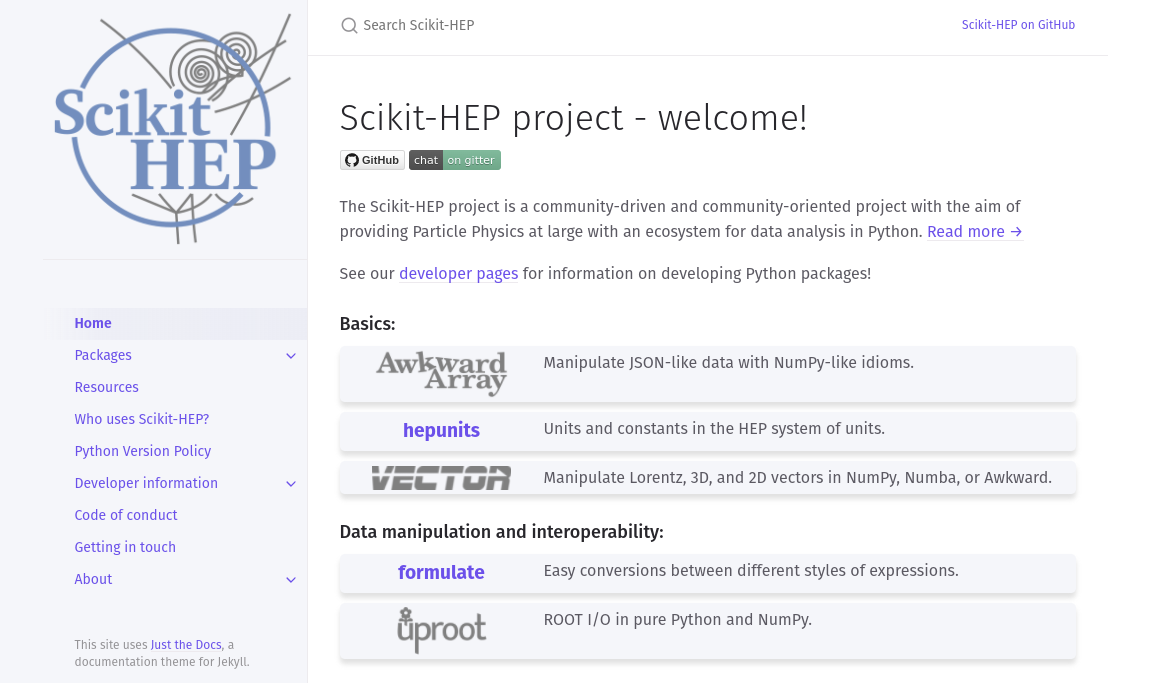
\includegraphics[width=\linewidth]{scikit-hep-webpage.png}
\end{columns}
\end{frame}

\begin{frame}{Stacked download statistics for Scikit-HEP and related packages}
\begin{columns}
\column{1.15\linewidth}
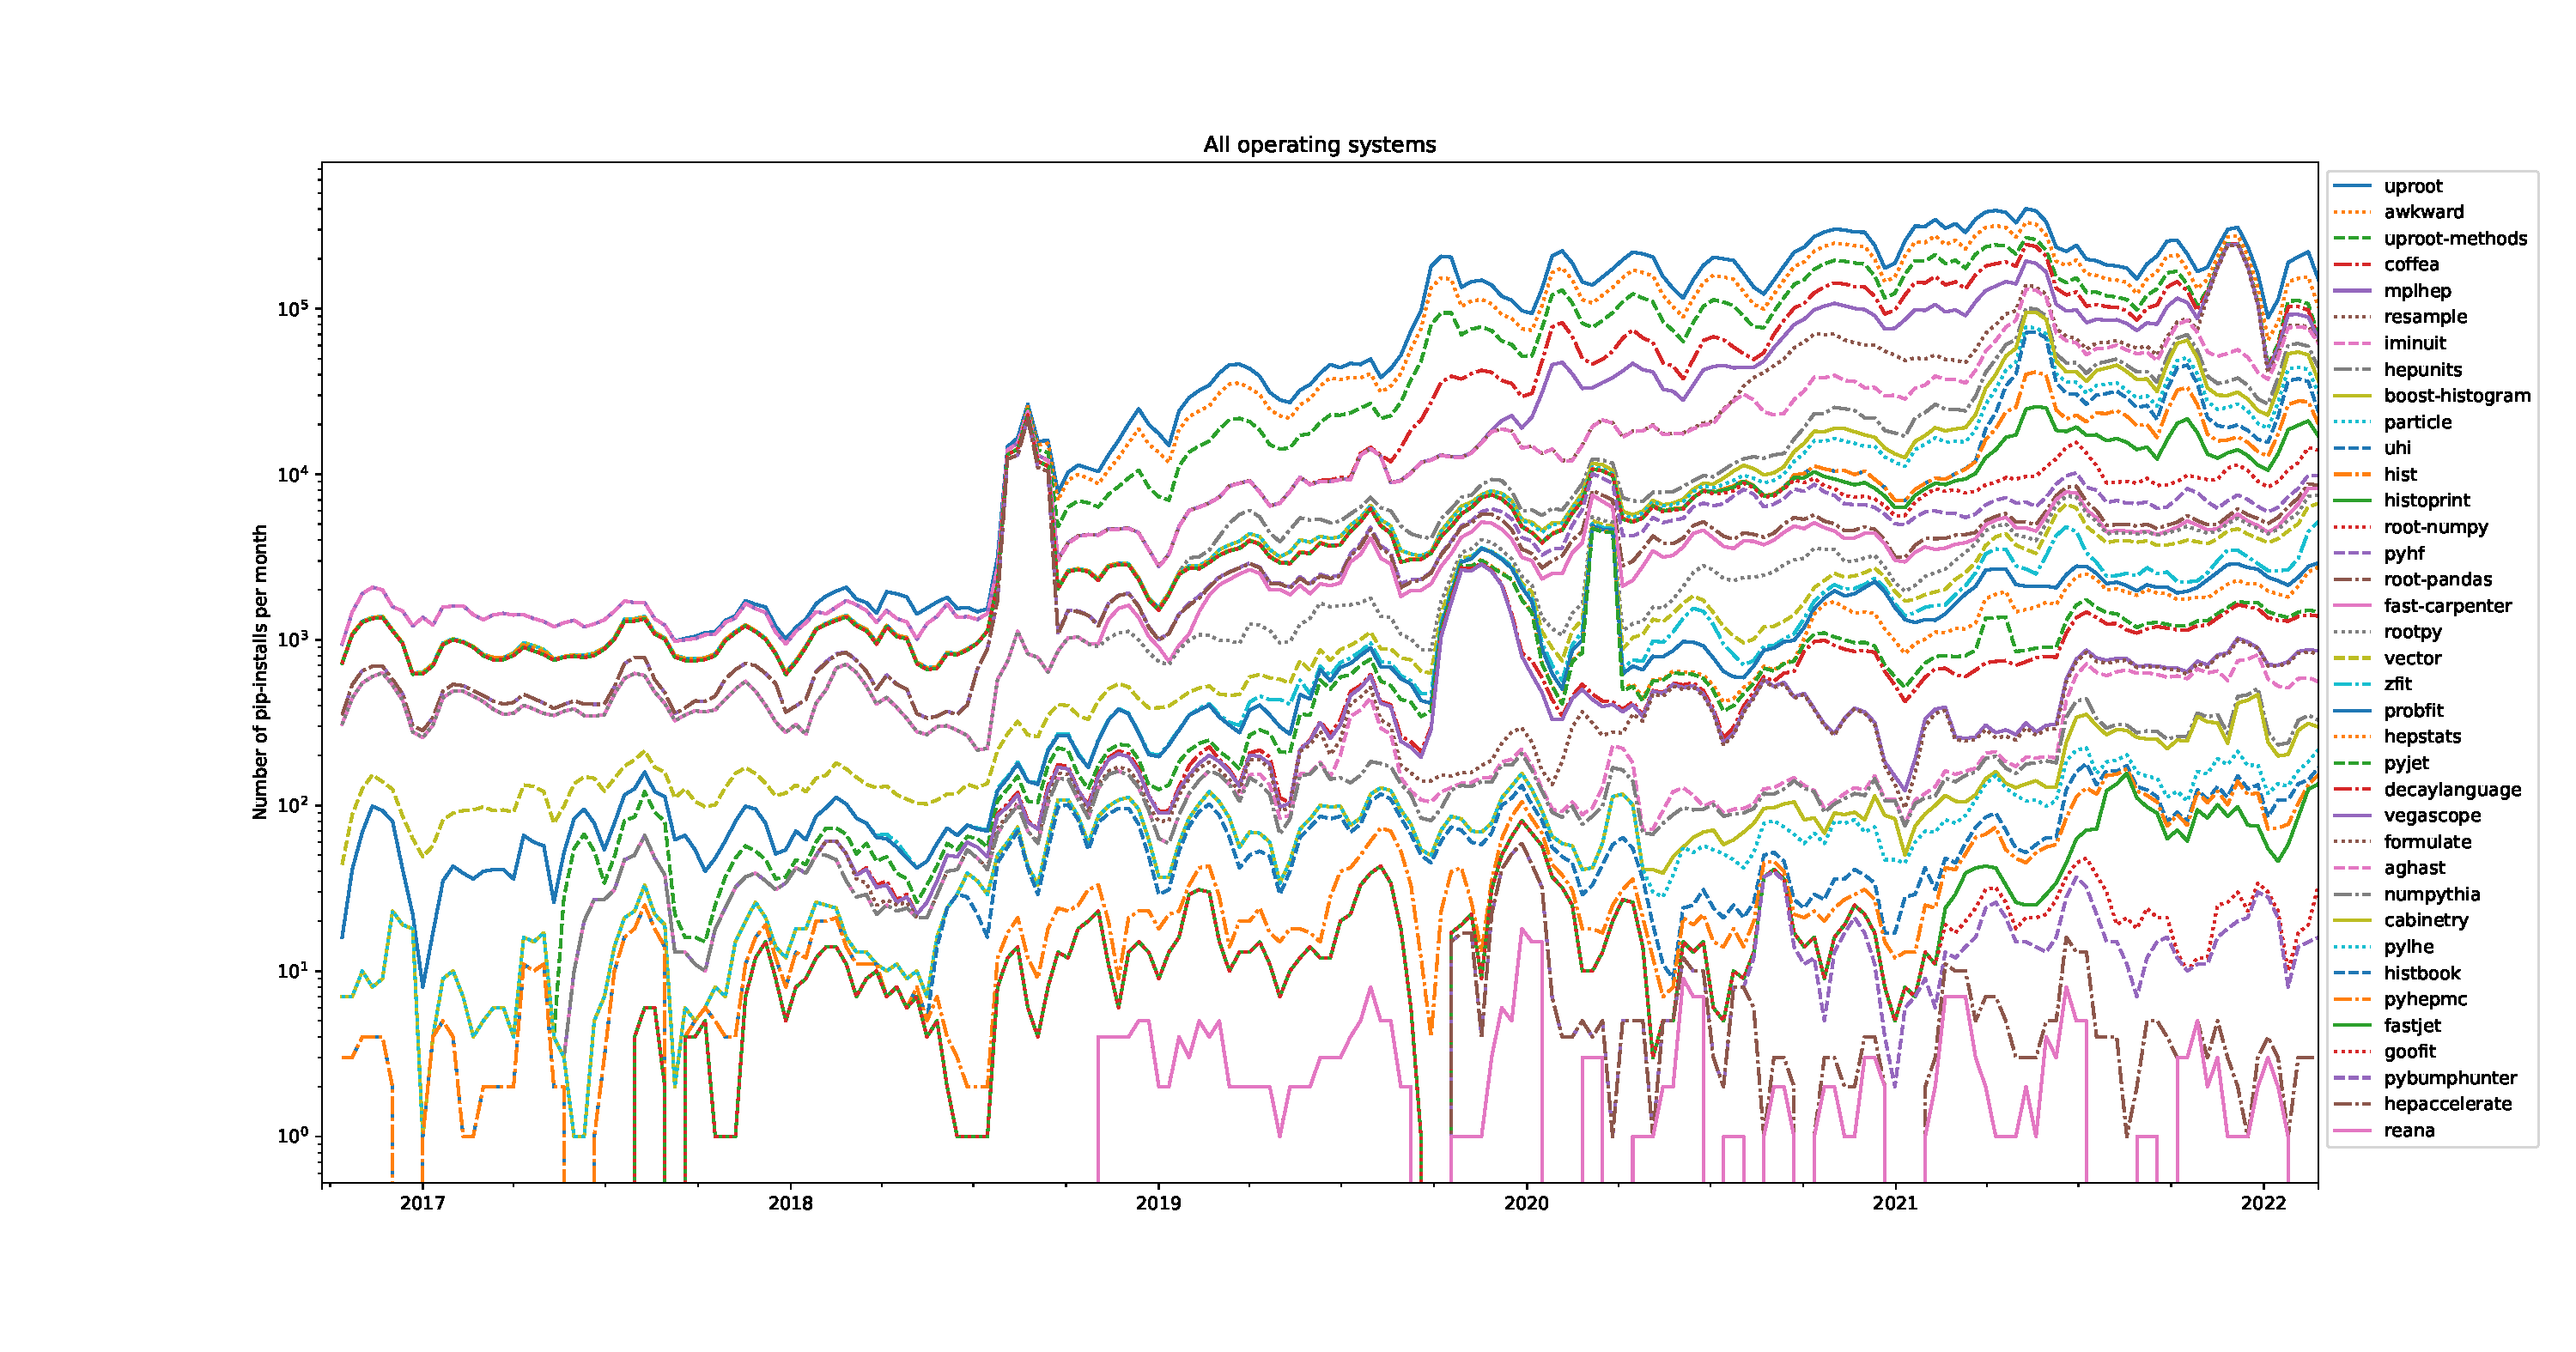
\includegraphics[width=\linewidth]{pip-allos-scikithep-log.pdf}
\end{columns}
\end{frame}

\begin{frame}{Learning about user needs: very different from my expectations!}
\vspace{0.25 cm}
\begin{columns}
\column{1.12\linewidth}
\only<1>{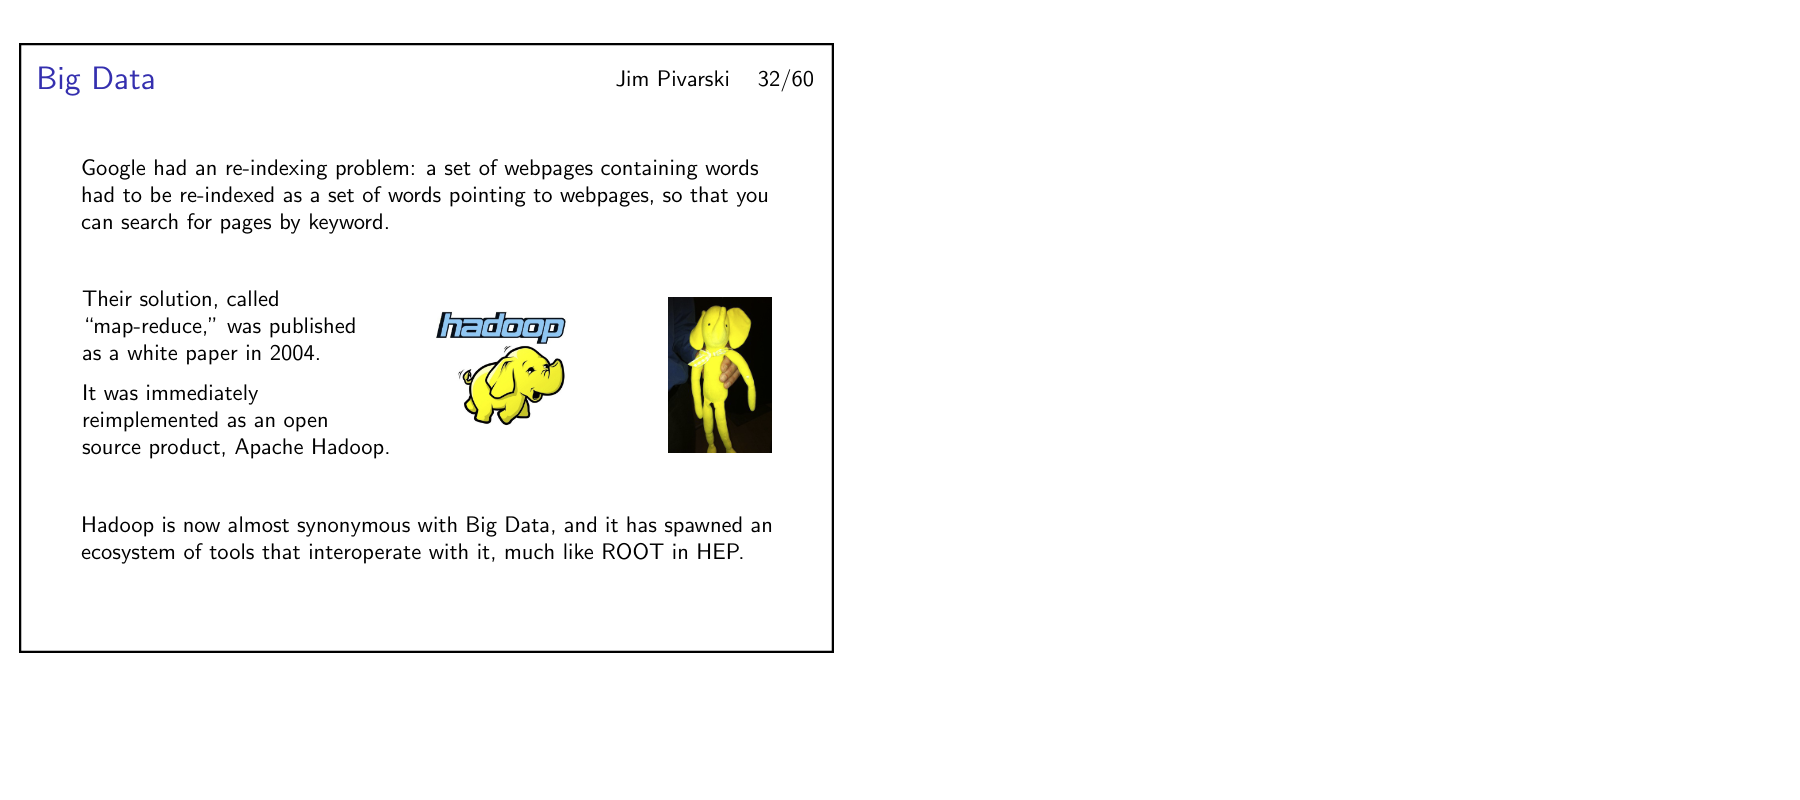
\includegraphics[width=\linewidth]{evolving-views-1.png}}\only<2>{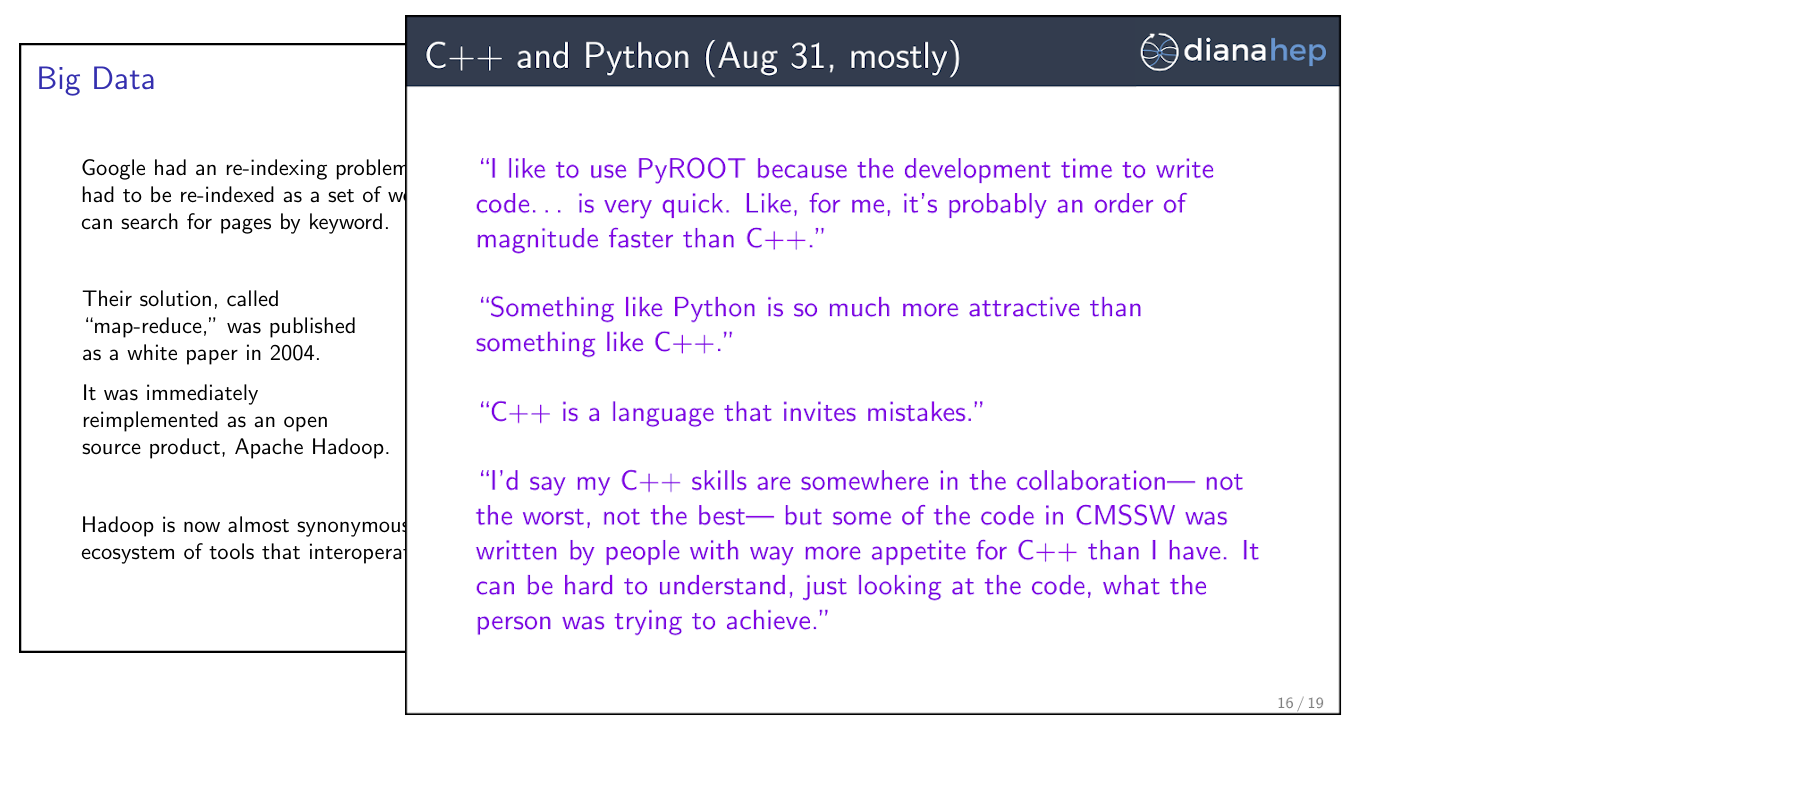
\includegraphics[width=\linewidth]{evolving-views-2.png}}\only<3>{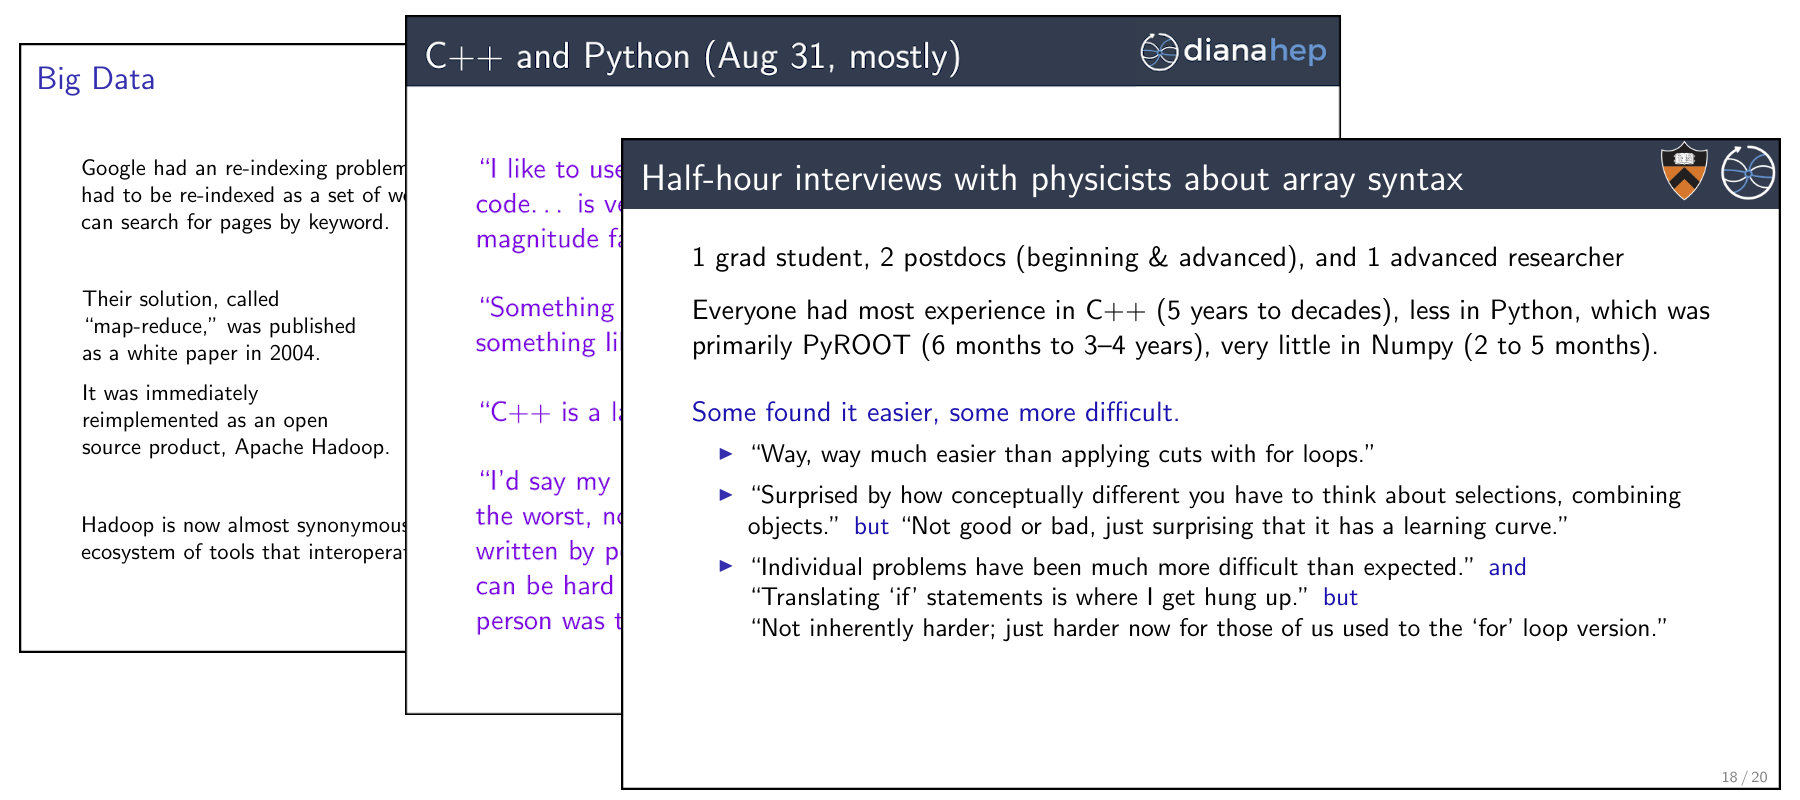
\includegraphics[width=\linewidth]{evolving-views-3.png}}\only<4>{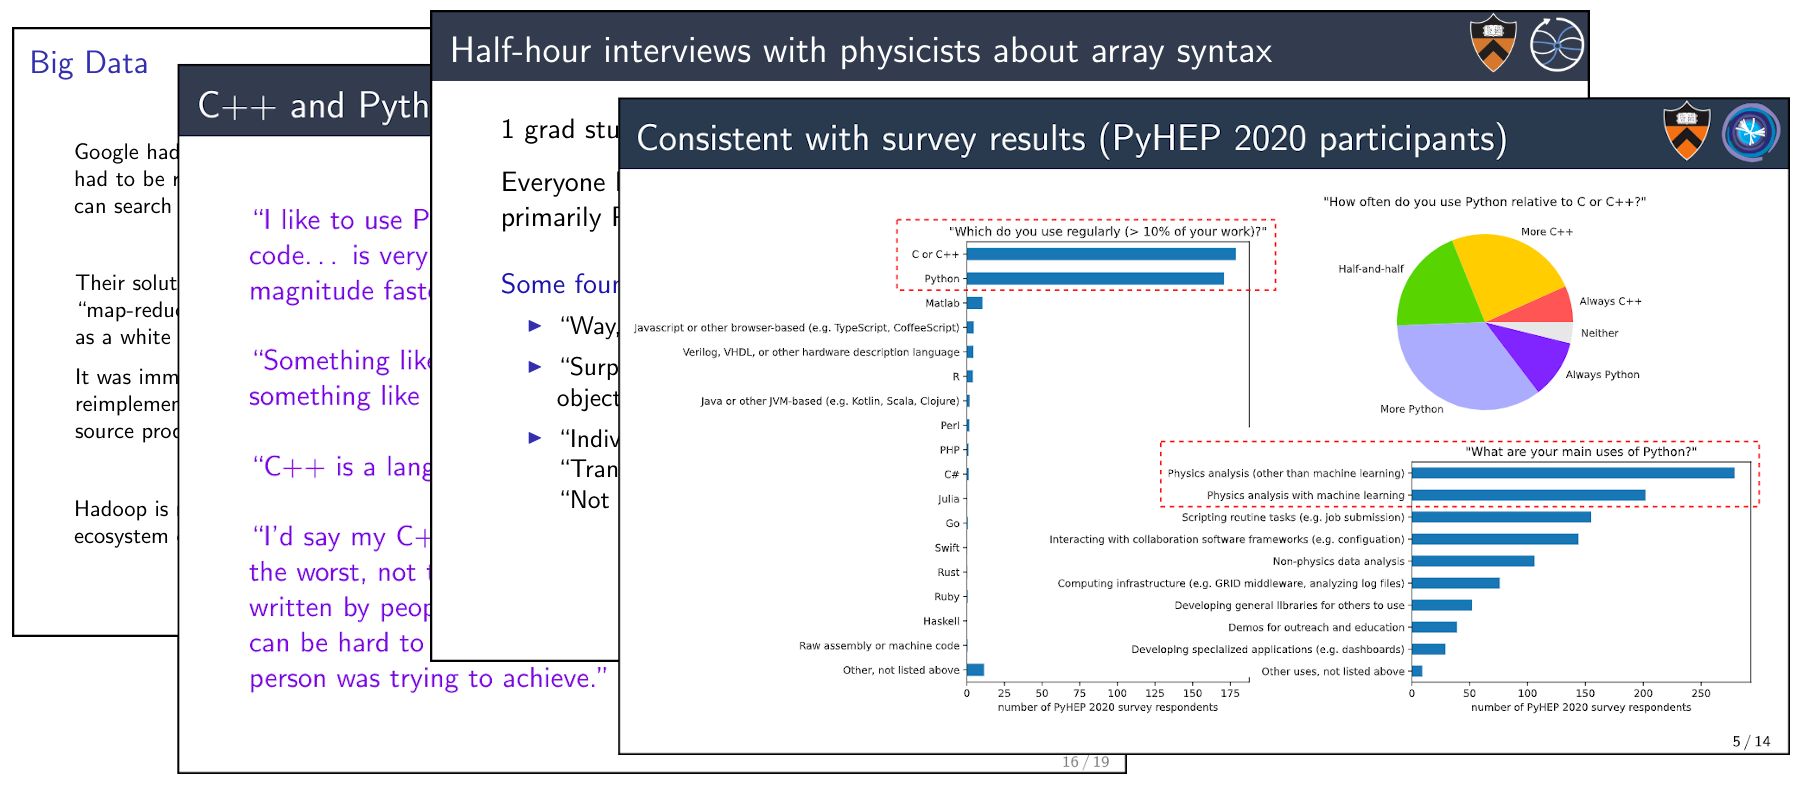
\includegraphics[width=\linewidth]{evolving-views-4.png}}
\end{columns}

\vspace{0.1 cm}
\uncover<2->{\Large\hfill Sought user input in focus groups, interviews, and surveys.}
\end{frame}

\begin{frame}{What I learned: now is the time to make HEP ``Pythonic''}
\vspace{0.22 cm}
\centering \only<1>{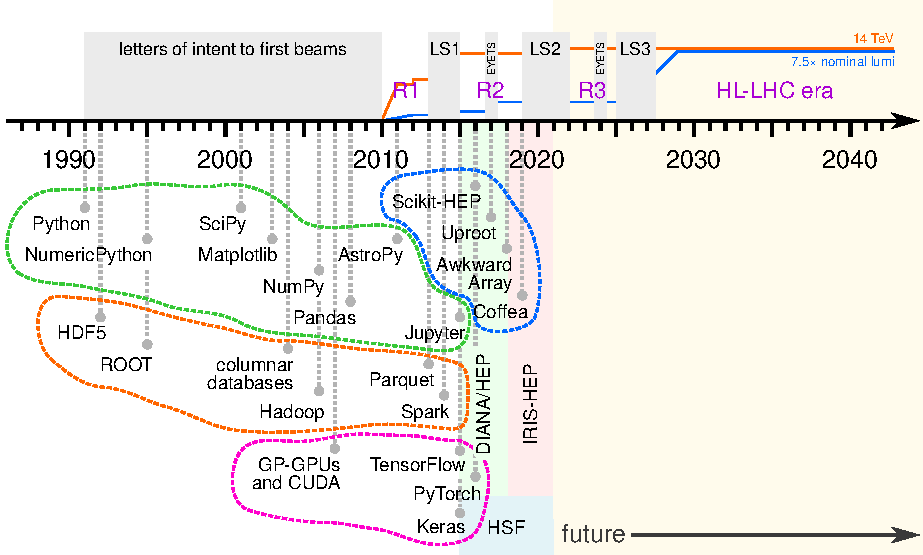
\includegraphics[width=0.92\linewidth]{hllhc-python-timeline-cloud-1.pdf}}\only<2>{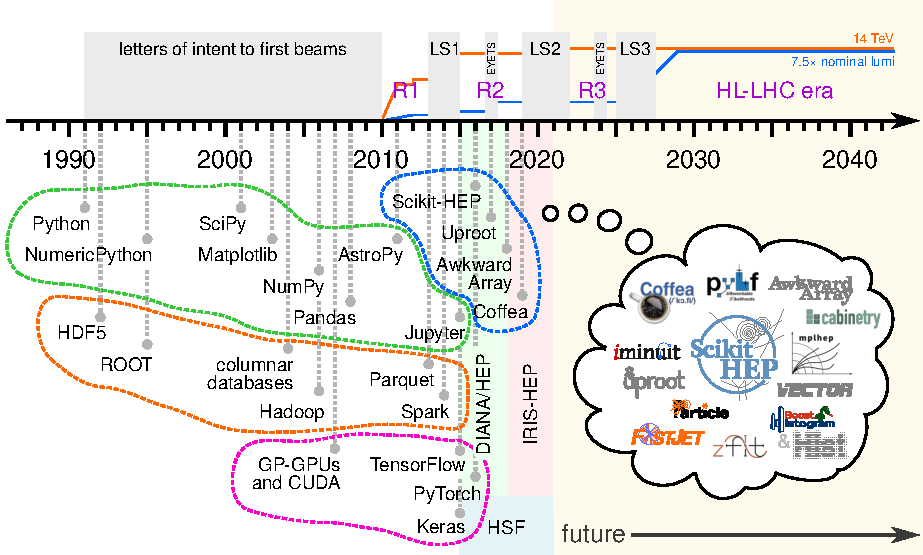
\includegraphics[width=0.92\linewidth]{hllhc-python-timeline-cloud-2.pdf}}
\end{frame}

\begin{frame}{Why Python? Why now?}
\large
\vspace{0.25 cm}
\textcolor{darkblue}{\mbox{\hspace{-0.5 cm}}Python is currently leading every ``most popular programming language'' index}

\vspace{0.25 cm}
\begin{columns}[t]
\column{0.33\linewidth}
\centering Tiobe

\vspace{0.1 cm}
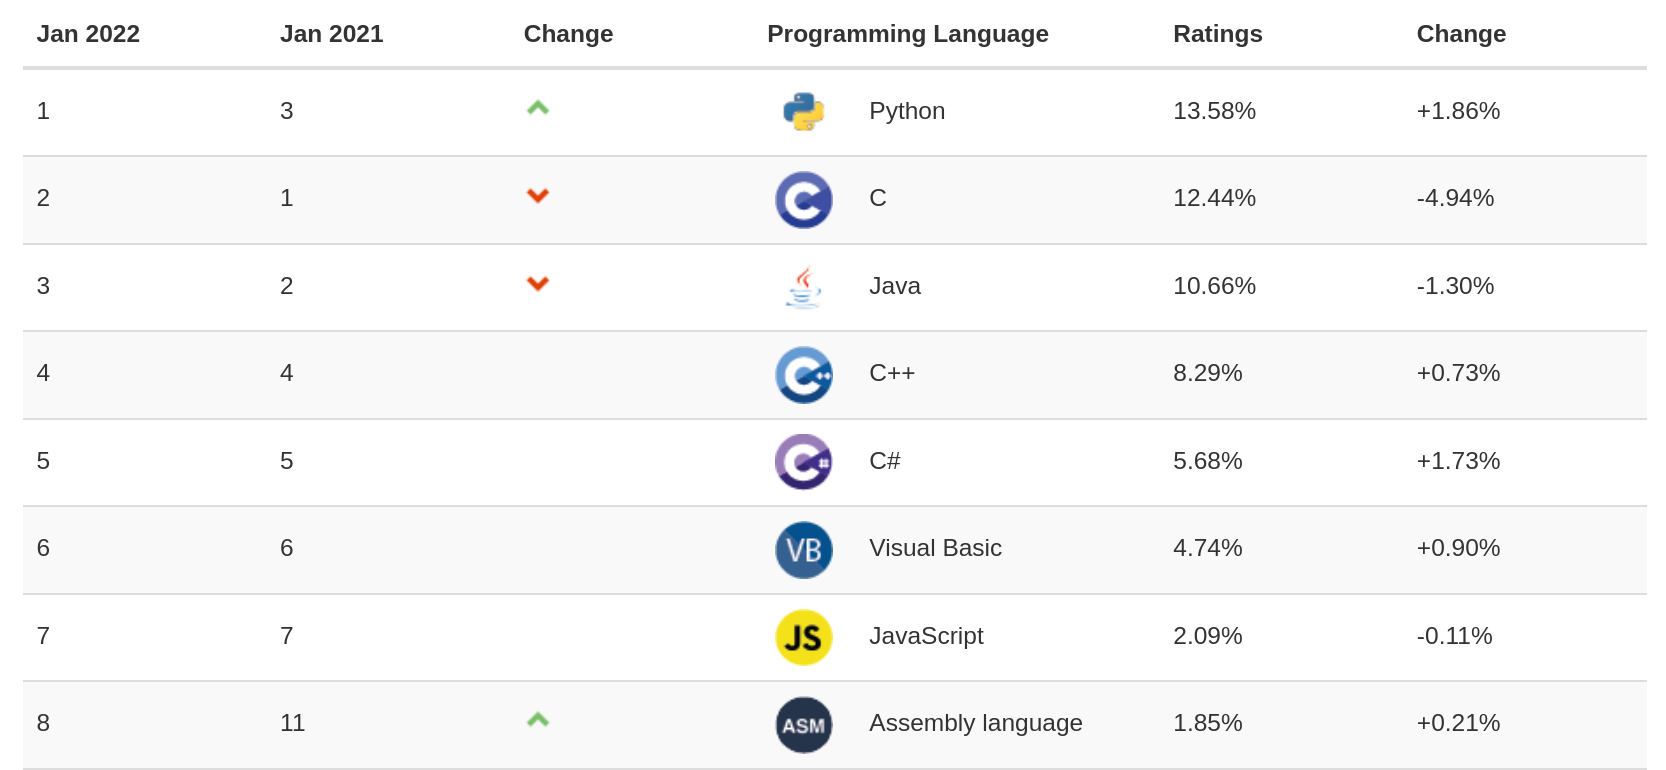
\includegraphics[width=\linewidth]{python-rankings-tiobe-2022.png}

\column{0.33\linewidth}
\centering PYPL

\vspace{0.1 cm}
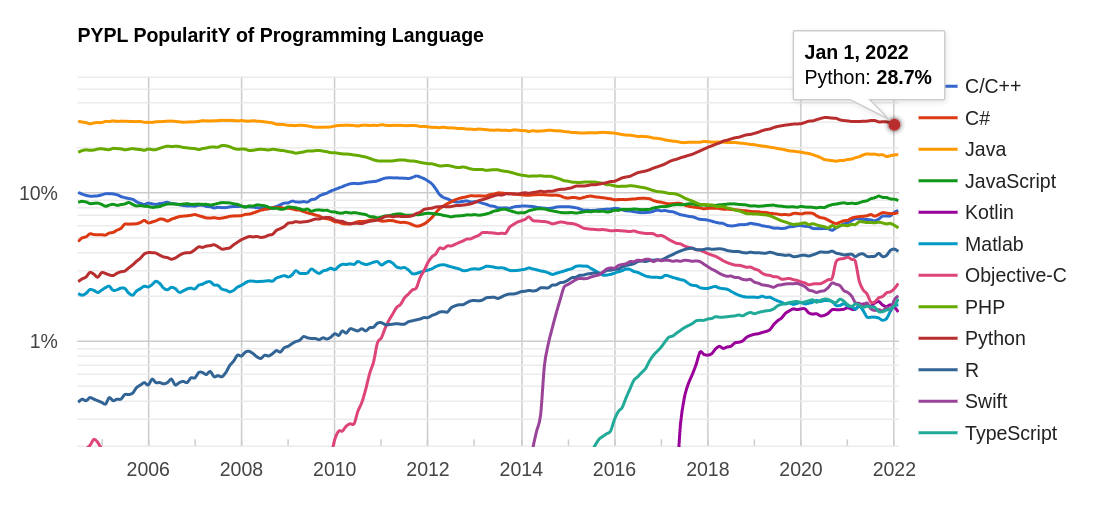
\includegraphics[width=\linewidth]{python-rankings-pypl-2022.png}

\column{0.33\linewidth}
\centering Google Trends

\vspace{0.1 cm}
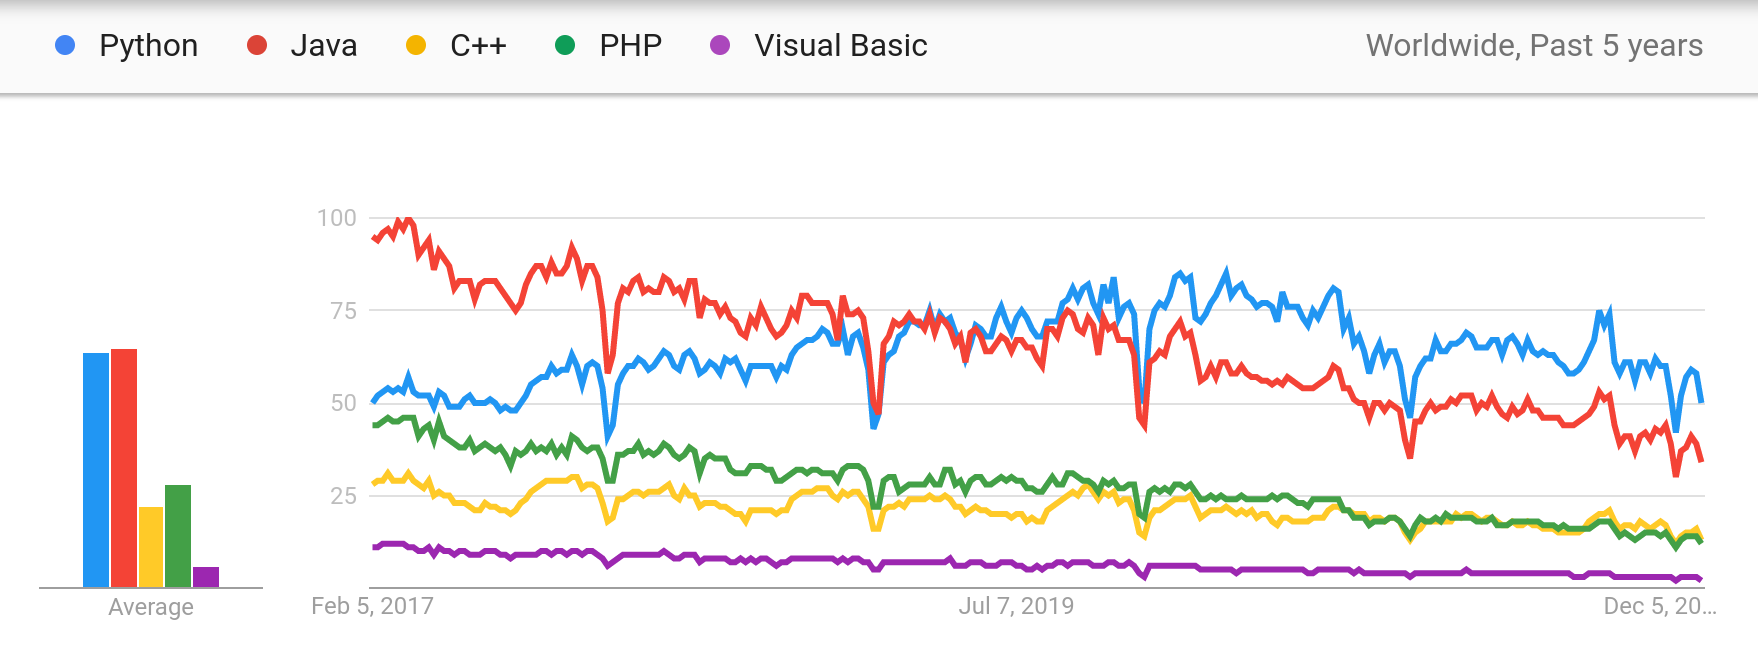
\includegraphics[width=\linewidth]{python-rankings-googletrends-2022.png}
\end{columns}

\vspace{0.25 cm}
\begin{columns}[t]
\column{0.5\linewidth}
\centering GitHut

\vspace{0.1 cm}
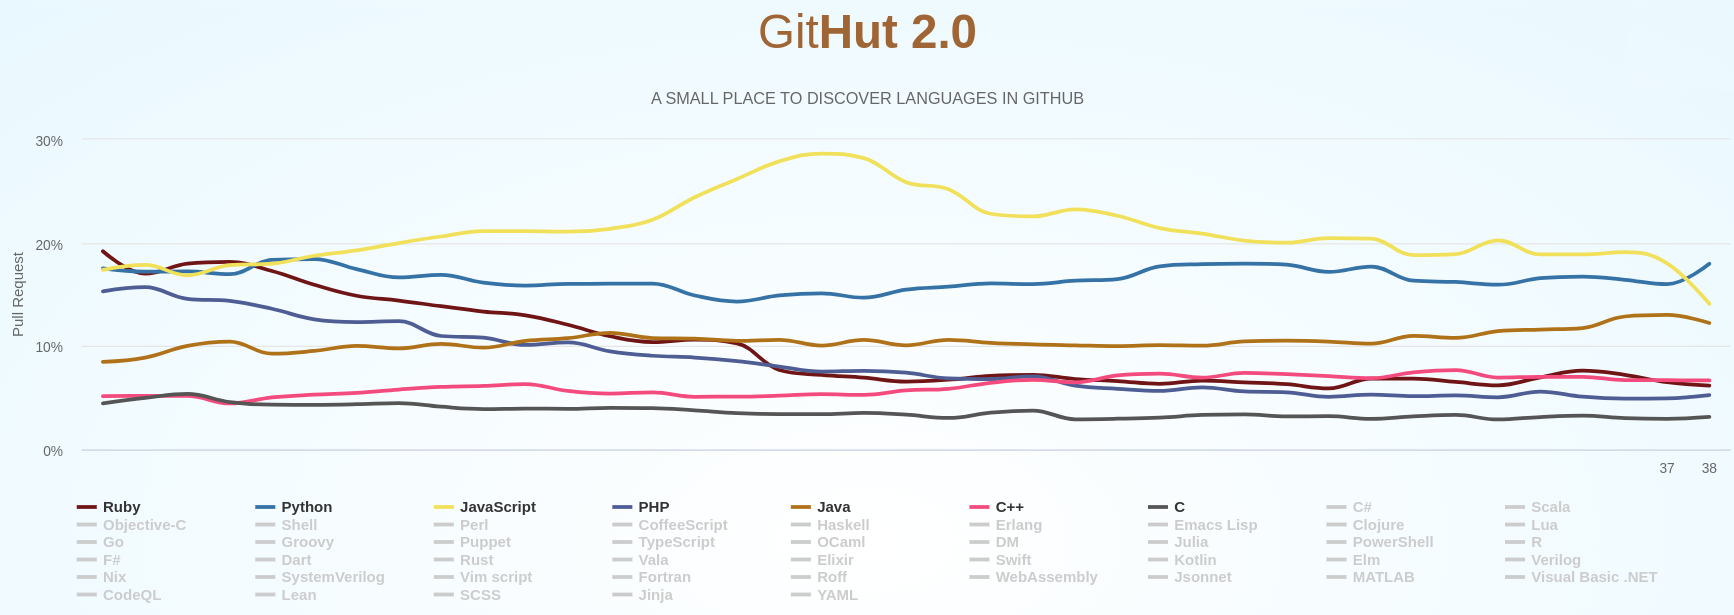
\includegraphics[width=\linewidth]{python-rankings-githut-2022.png}

\column{0.45\linewidth}
\centering StackOverflow

\vspace{0.1 cm}
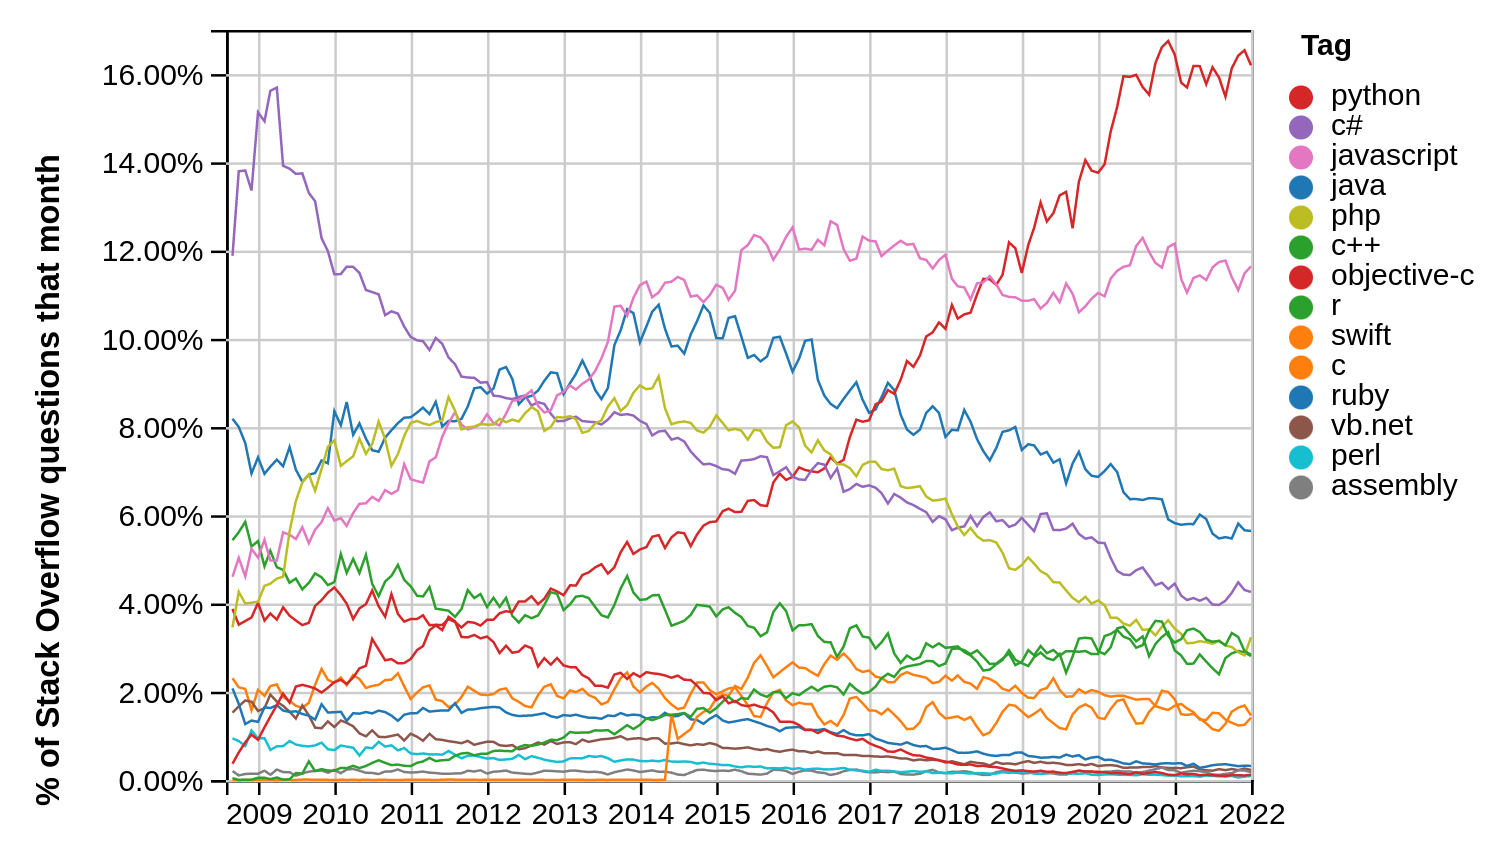
\includegraphics[width=\linewidth]{python-rankings-stackoverflow-2022.png}
\end{columns}
\end{frame}

\begin{frame}{Why Python? Why now?}
\large
\vspace{0.25 cm}
\textcolor{darkblue}{\mbox{\hspace{-0.5 cm}}Especially in data analysis (below: coincidence of search terms in Google Trends)}

\vspace{0.15 cm}
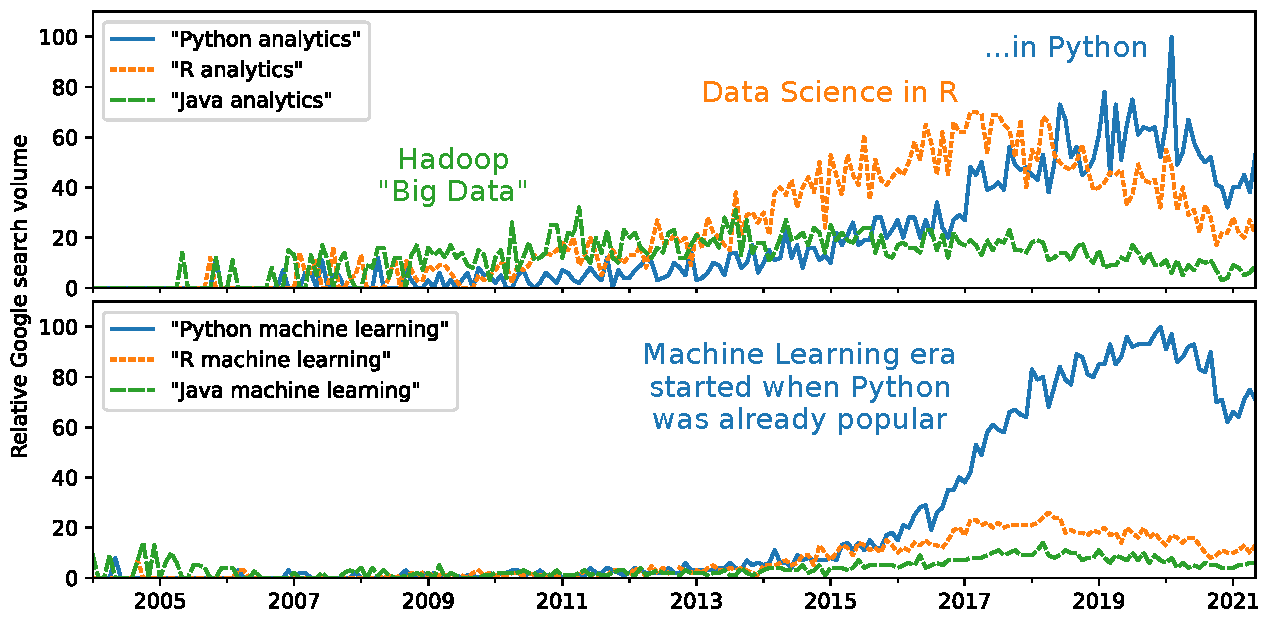
\includegraphics[width=\linewidth]{analytics-by-language.pdf}
\end{frame}

\begin{frame}{Python has also been relevant in HEP {\it for 20 years}}
\vspace{0.25 cm}
\textcolor{darkblue}{\mbox{\hspace{-0.5 cm}}Programming languages mentioned in CHEP \uncover<2->{and ACAT (this one is not as clear)}}

\vspace{-0.03 cm}
\begin{columns}
\column{1.08\linewidth}
\only<1>{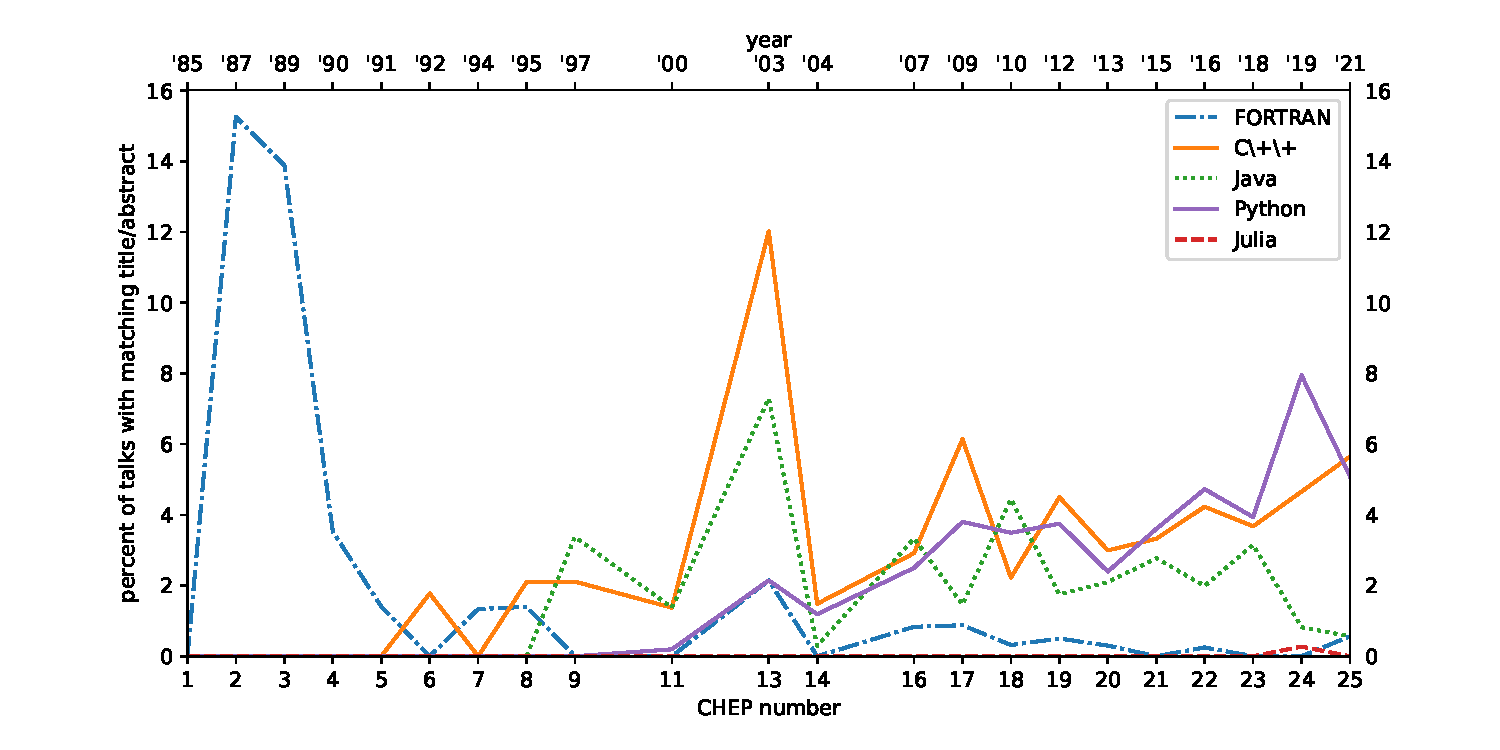
\includegraphics[width=\linewidth]{chep-papers-language-2.pdf}}\only<2>{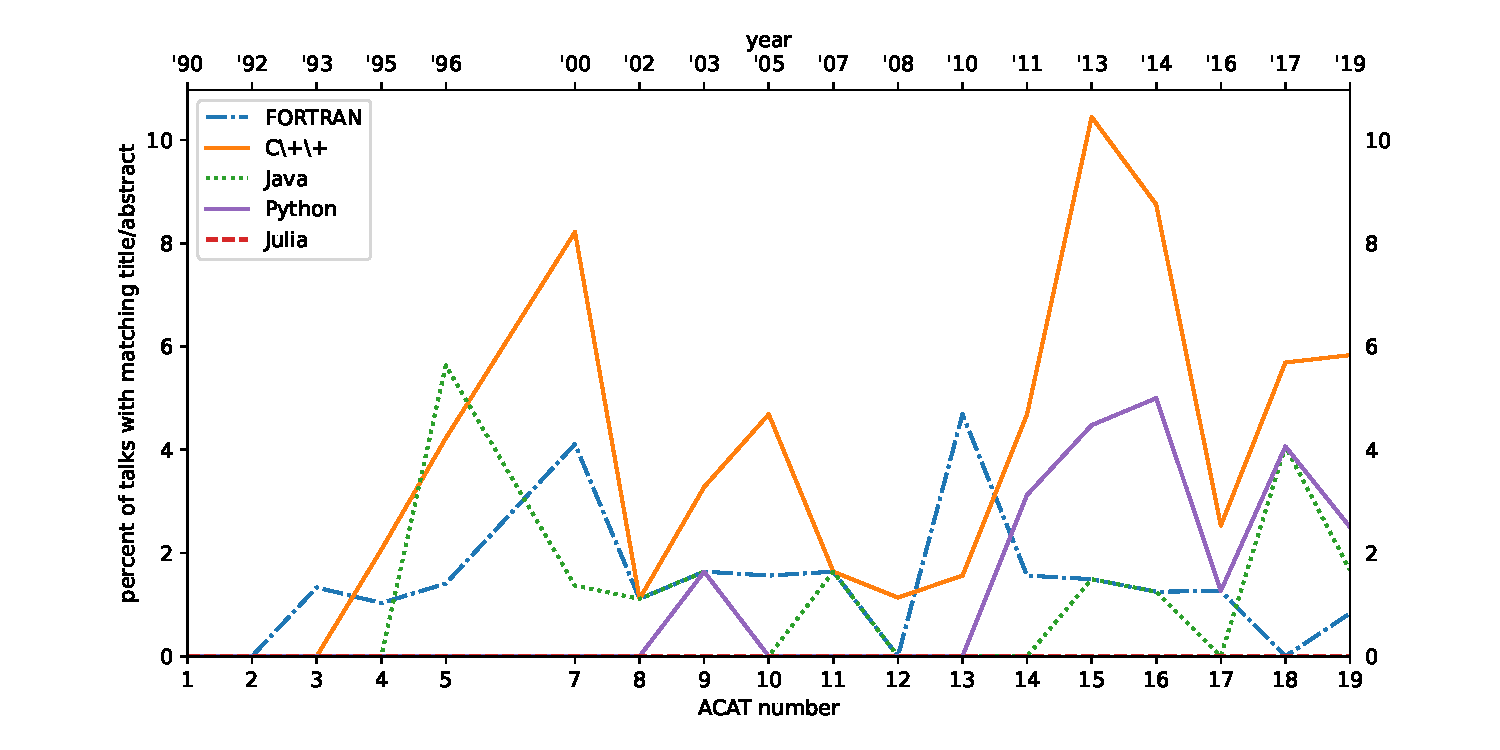
\includegraphics[width=\linewidth]{acat-papers-language-2.pdf}}
\end{columns}
\end{frame}

\begin{frame}{Lucas Taylor, {\it Summary of Data Analysis Track,} CHEP 2001}
\vspace{0.25 cm}
\begin{columns}
\column{0.05\linewidth}

\column{0.81\linewidth}
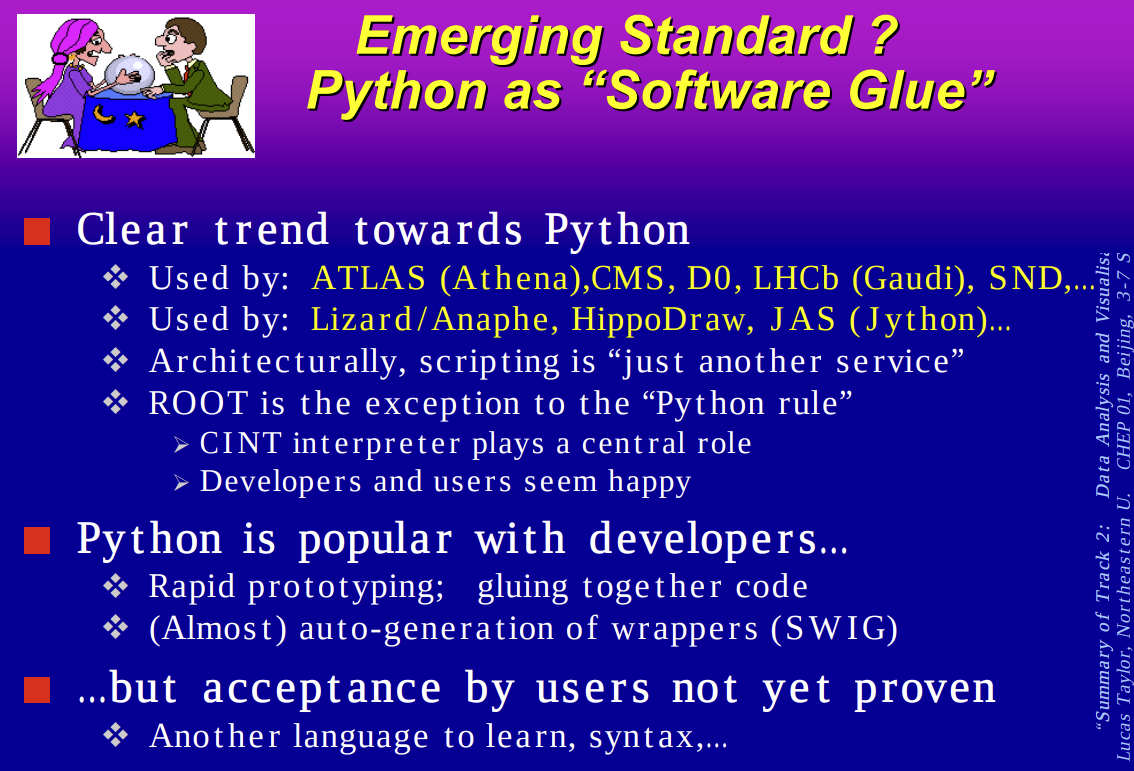
\includegraphics[width=\linewidth]{chep-2001-python.png}

\column{0.2\linewidth}
Note: PyROOT introduced in 2004 (v4.00/04).
\end{columns}
\end{frame}

\begin{frame}{Much longer than the resurgence of interest in machine learning}
\vspace{0.25 cm}
\textcolor{darkblue}{\mbox{\hspace{-0.5 cm}}Machine learning terms mentioned in CHEP \uncover<2->{and ACAT}}

\vspace{-0.03 cm}
\begin{columns}
\column{1.08\linewidth}
\only<1>{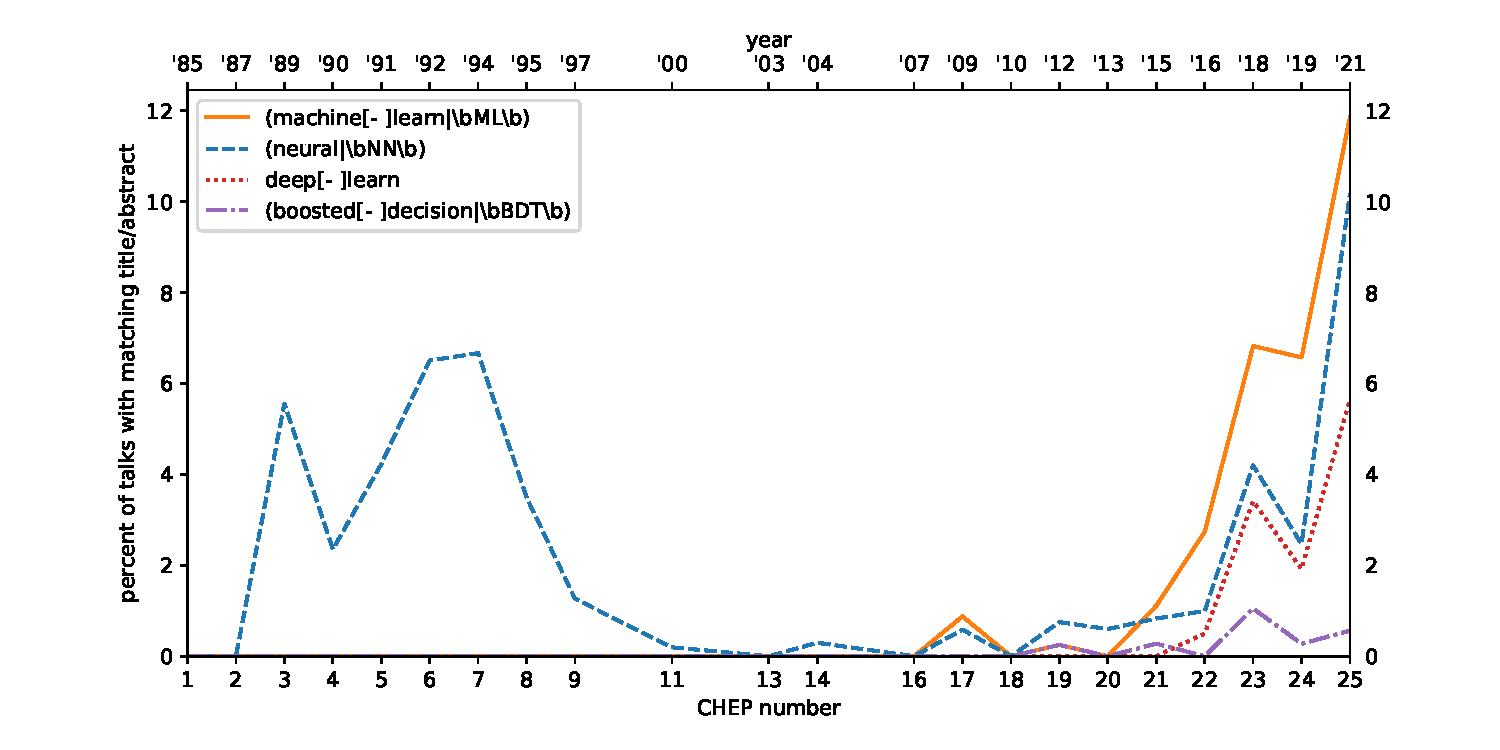
\includegraphics[width=\linewidth]{chep-papers-ml.pdf}}\only<2>{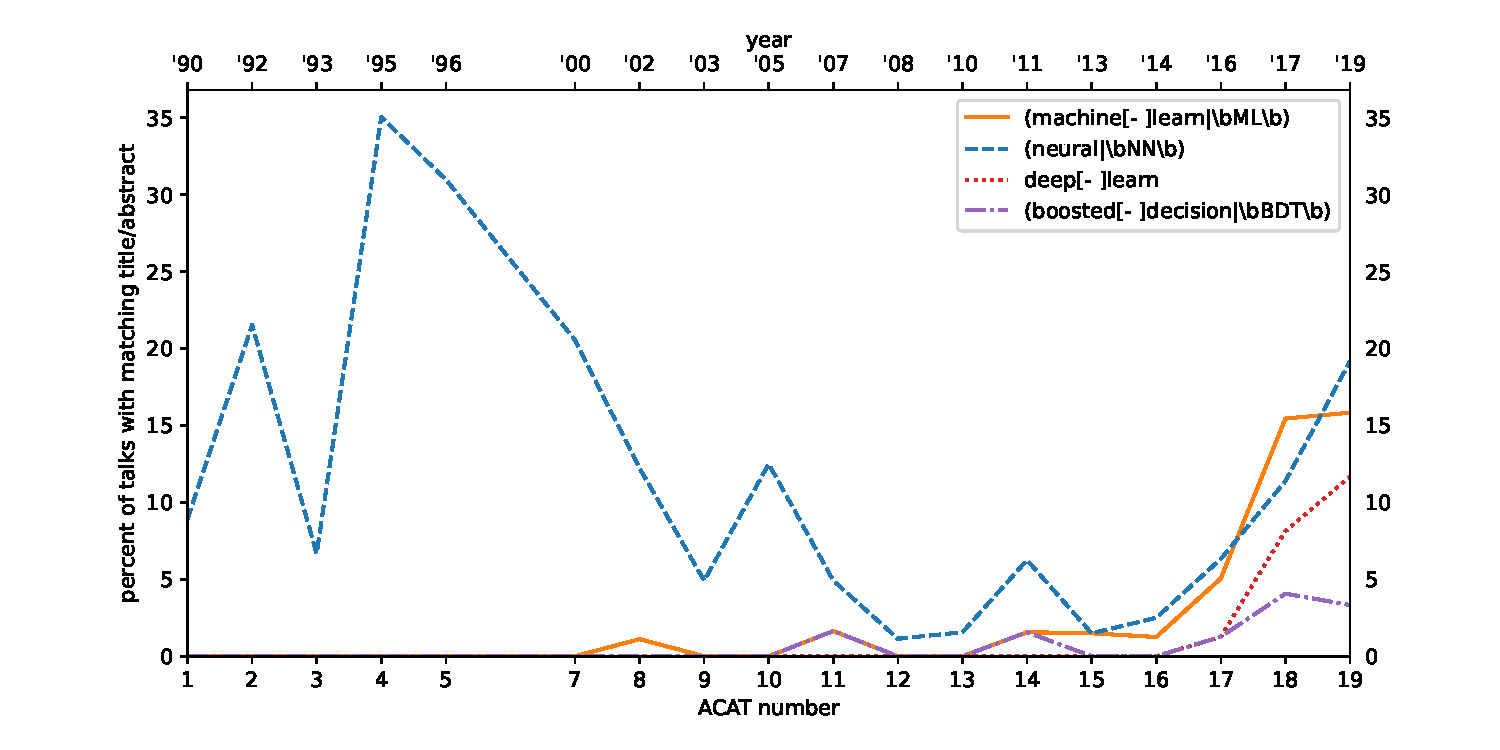
\includegraphics[width=\linewidth]{acat-papers-ml.pdf}}
\end{columns}
\end{frame}

\begin{frame}{How is Python being used by physicists?}
\vspace{0.5 cm}
{\Large Analyze code in 11\,635 GitHub repos written by 2\,172 physicists:}

\vspace{0.25 cm}
\begin{enumerate}
\item Ask GitHub which users forked CMSSW and call them ``CMS physicists.'' (CMSSW has been on GitHub for a long enough time to see trends.)
\item Clone all of the physicists' repos (the ones that are not forks of something else).
\item Search the code of these repos and count matches.
\item Take care to exclude CMSSW configuration files, which are also Python.
\end{enumerate}

\begin{center}
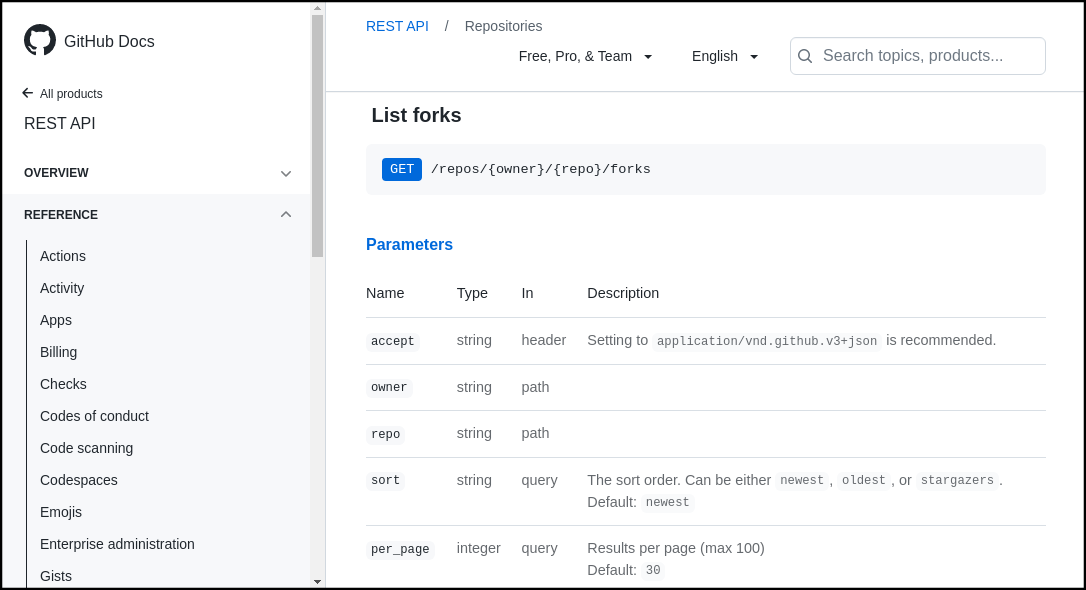
\includegraphics[width=0.5\linewidth]{github-api-website.png}
\end{center}
\end{frame}

\begin{frame}{How is Python being used by physicists?}
\vspace{0.25 cm}
\textcolor{darkblue}{\mbox{\hspace{-0.5 cm}}\only<1>{Number of non-fork GitHub repos created by CMS physicists (users who forked CMSSW)}\only<2>{Same sample, now counting regex matches for \mintinline{python}{import XYZ}, \mintinline{python}{from XYZ import}, etc.}}

\vspace{-0.35 cm}
\begin{columns}
\column{1.15\linewidth}
\only<1>{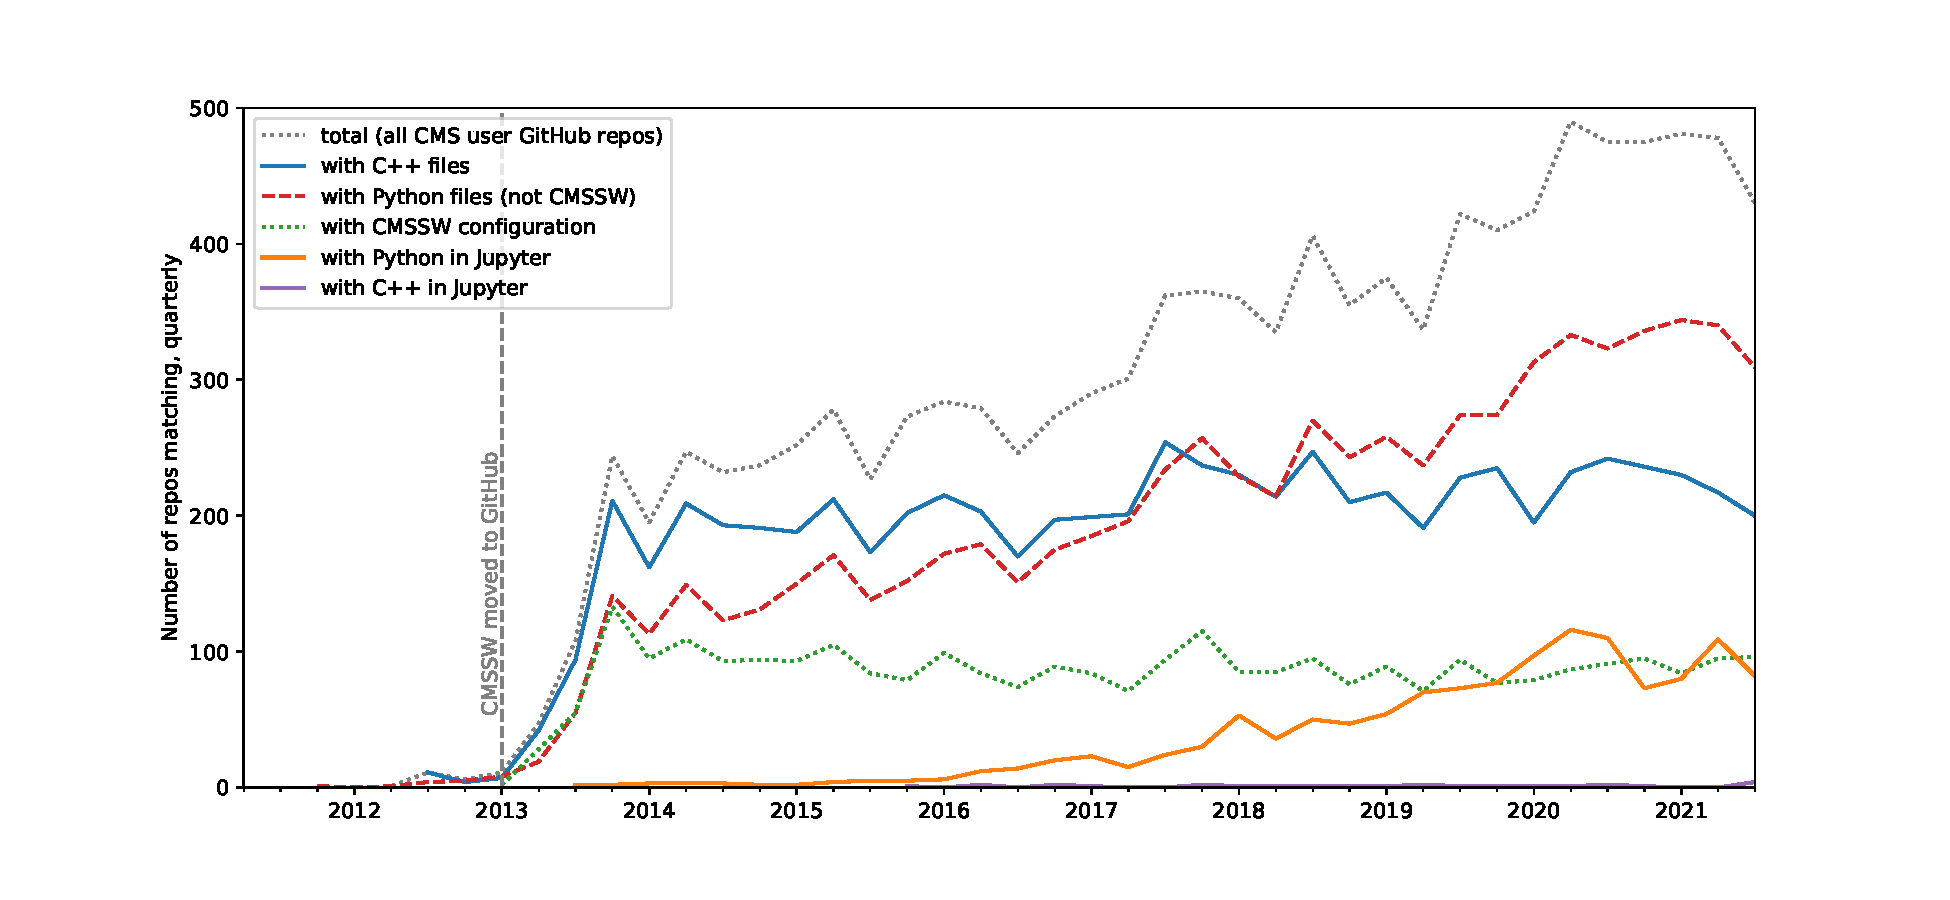
\includegraphics[width=\linewidth]{gihub-language-fullstudy.pdf}}\only<2>{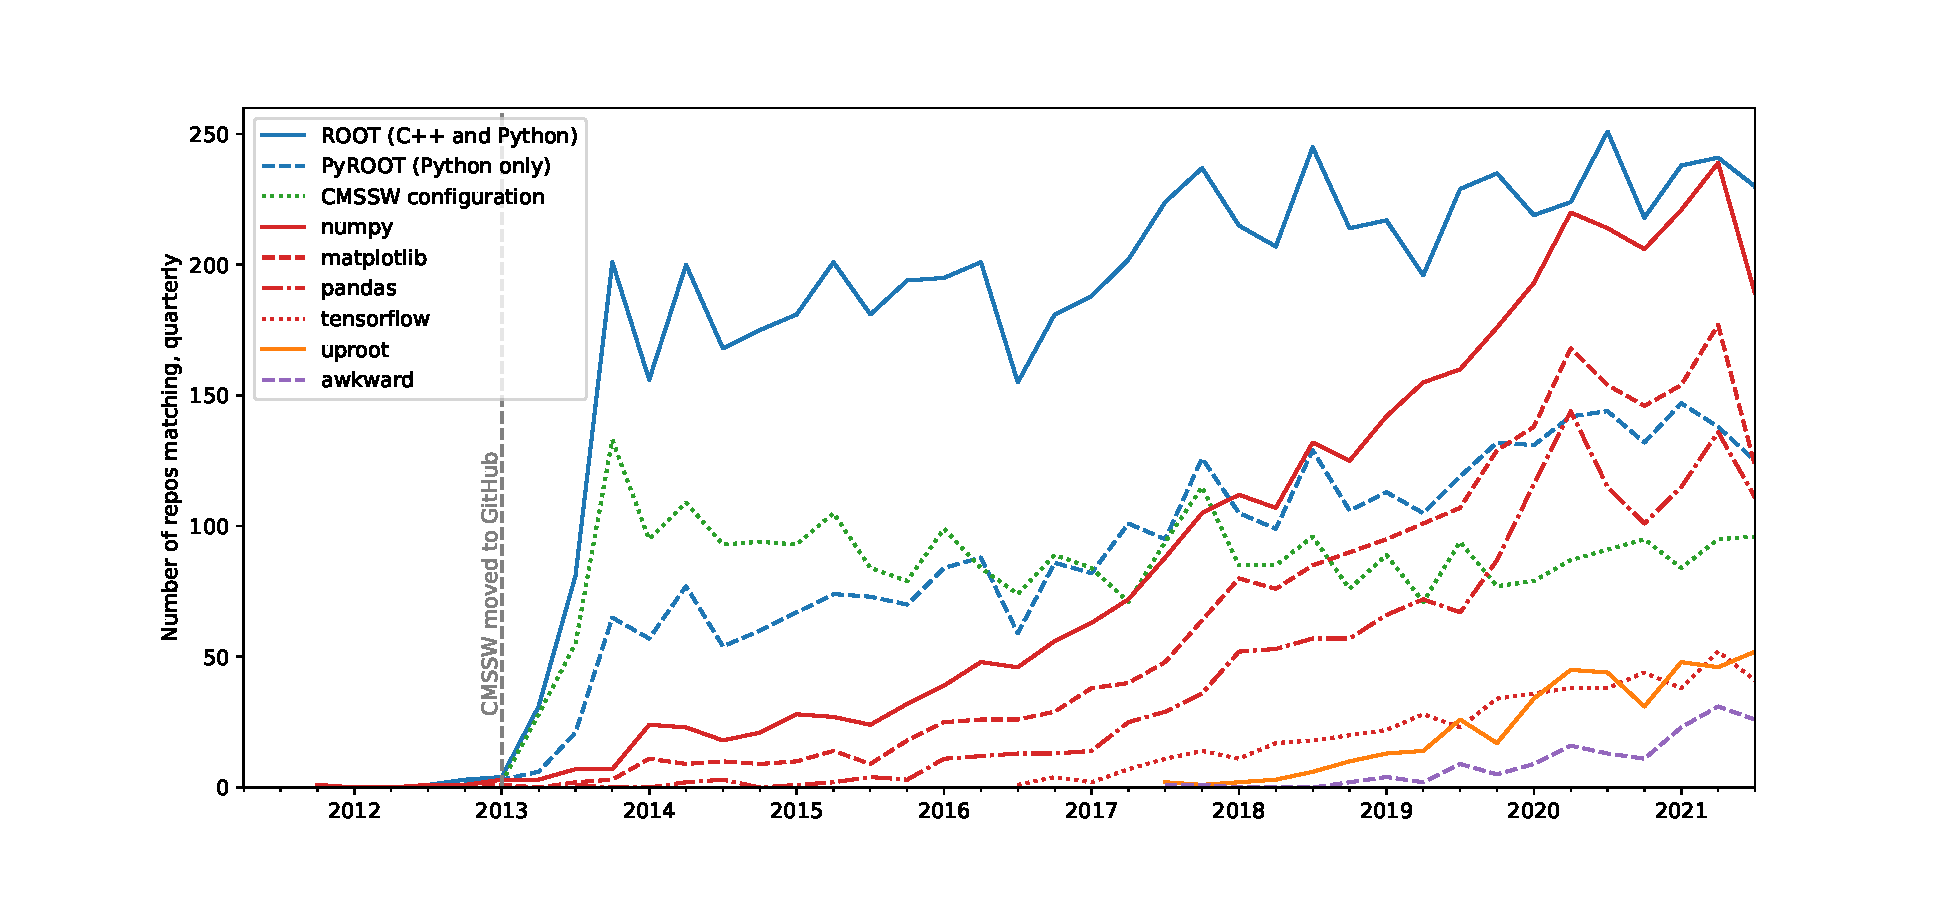
\includegraphics[width=\linewidth]{gihub-package-fullstudy.pdf}}
\end{columns}
\end{frame}

\begin{frame}{Conclusions}
\large
\begin{itemize}\setlength{\itemsep}{0.25 cm}
\item<1-> Python has been slowly growing in HEP for 20 years (unlike the ``big bang'' when C++ replaced Fortran).
\item<2-> But physicists started using the SciPy ecosystem (NumPy, Matplotlib, Pandas, etc.) about 5~years ago.
\item<3-> Scikit-HEP also started 5~years ago, just in time to serve this need.
\item<4-> C++, ROOT, and collaboration software configuations have been {\it steady}, while Python and the SciPy ecosystem have been {\it rising}.
\end{itemize}
\end{frame}

\begin{frame}{PyHEP 2020 survey respondents ($N=406$): same picture}
\vspace{0.2 cm}
\begin{columns}
\column{1.15\linewidth}
\only<1>{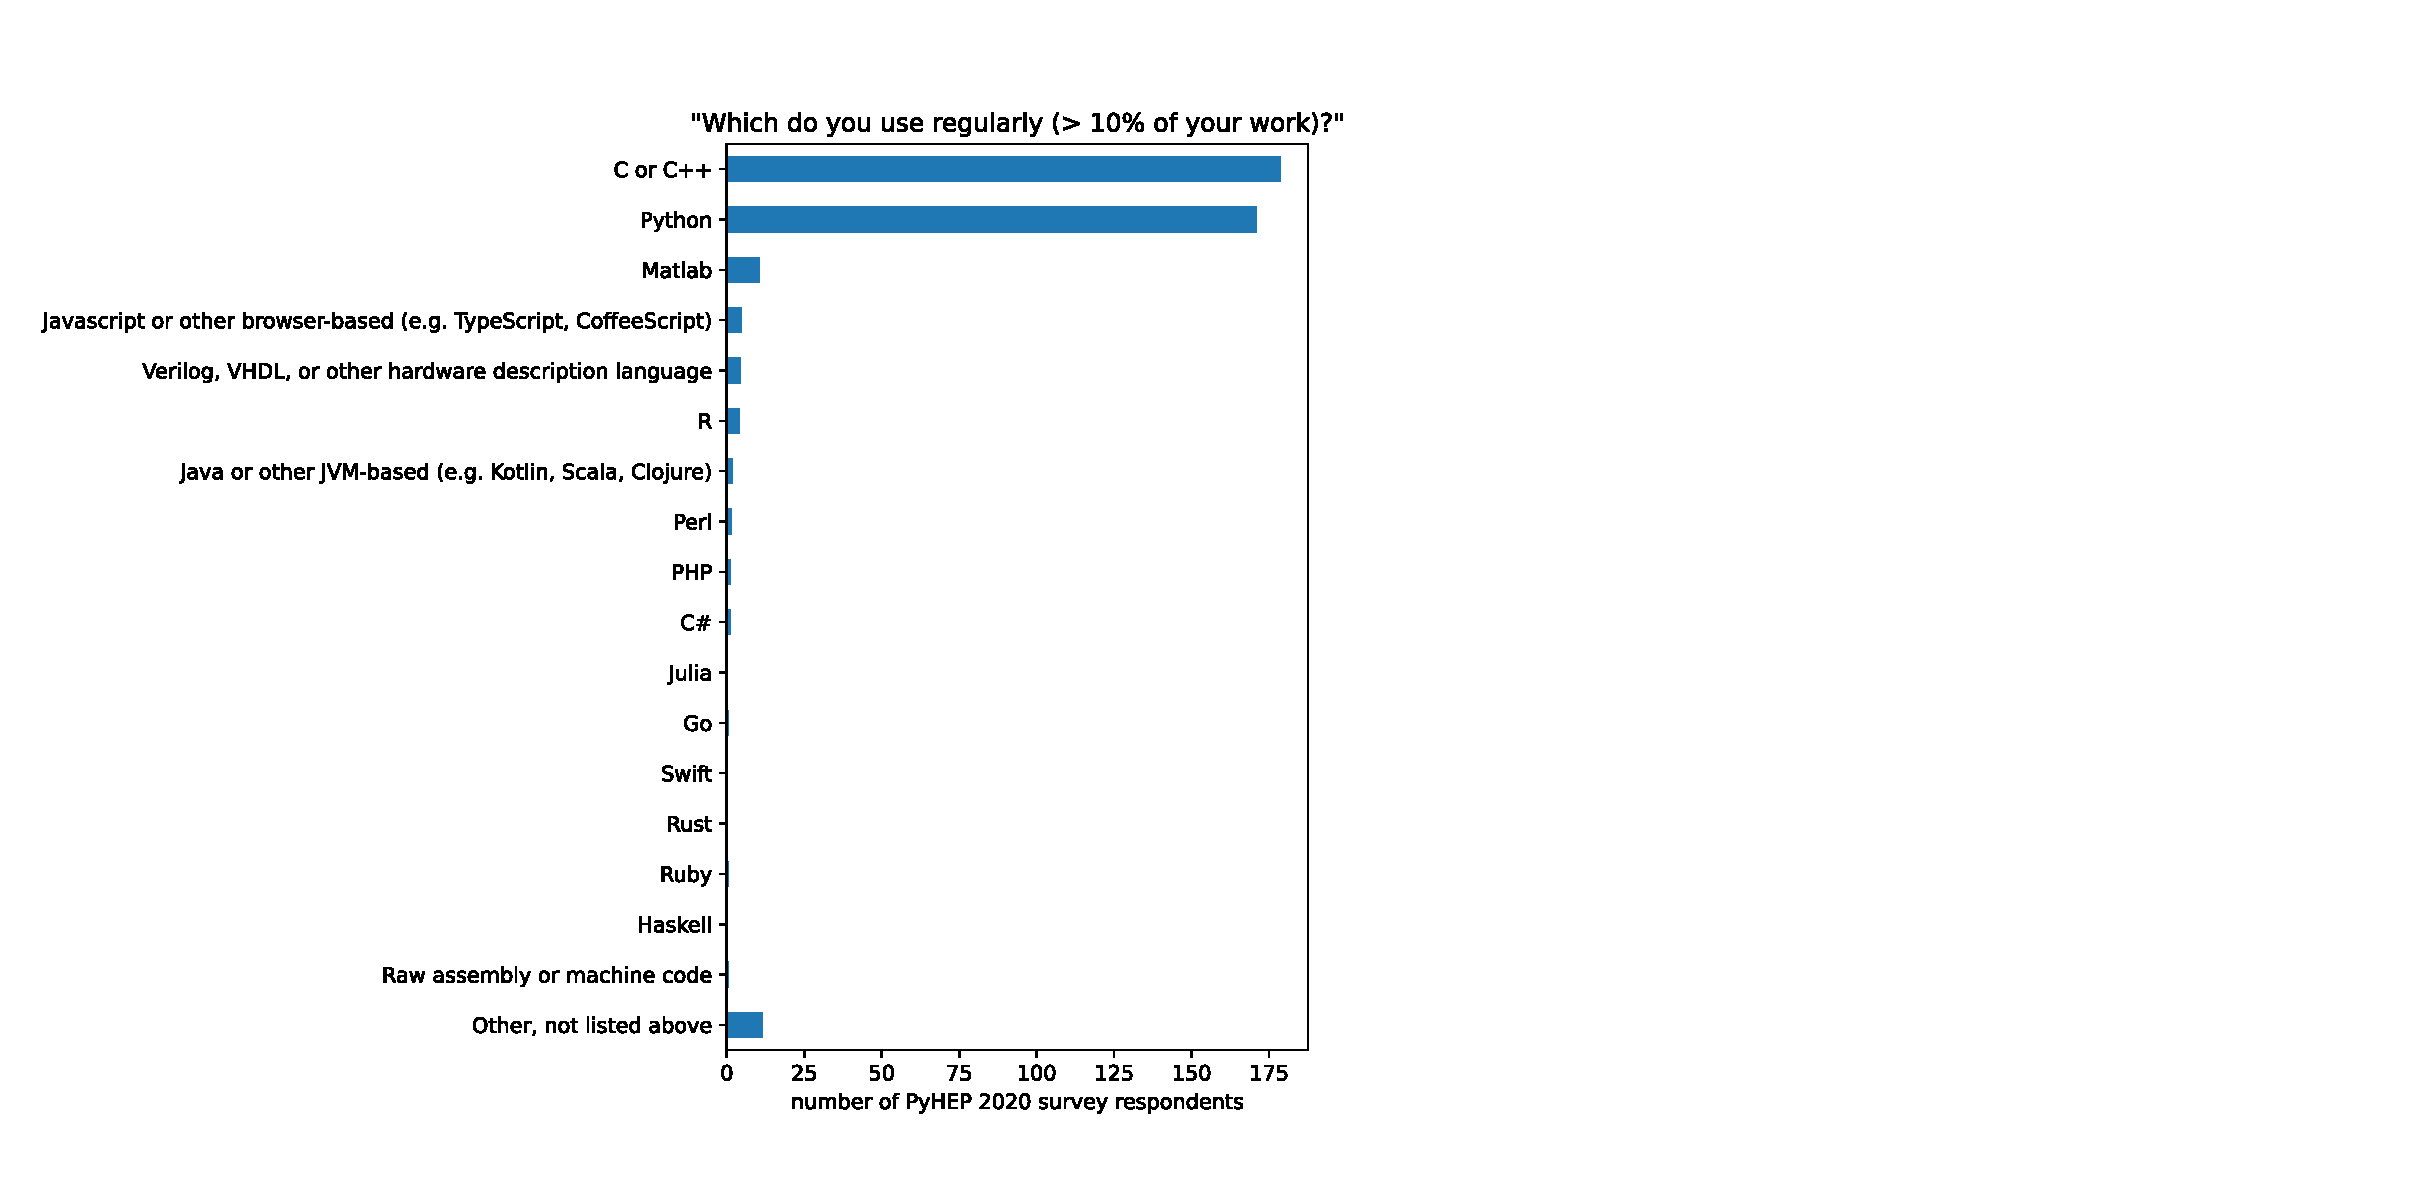
\includegraphics[width=\linewidth]{pyhep2020-survey-1.pdf}}\only<2>{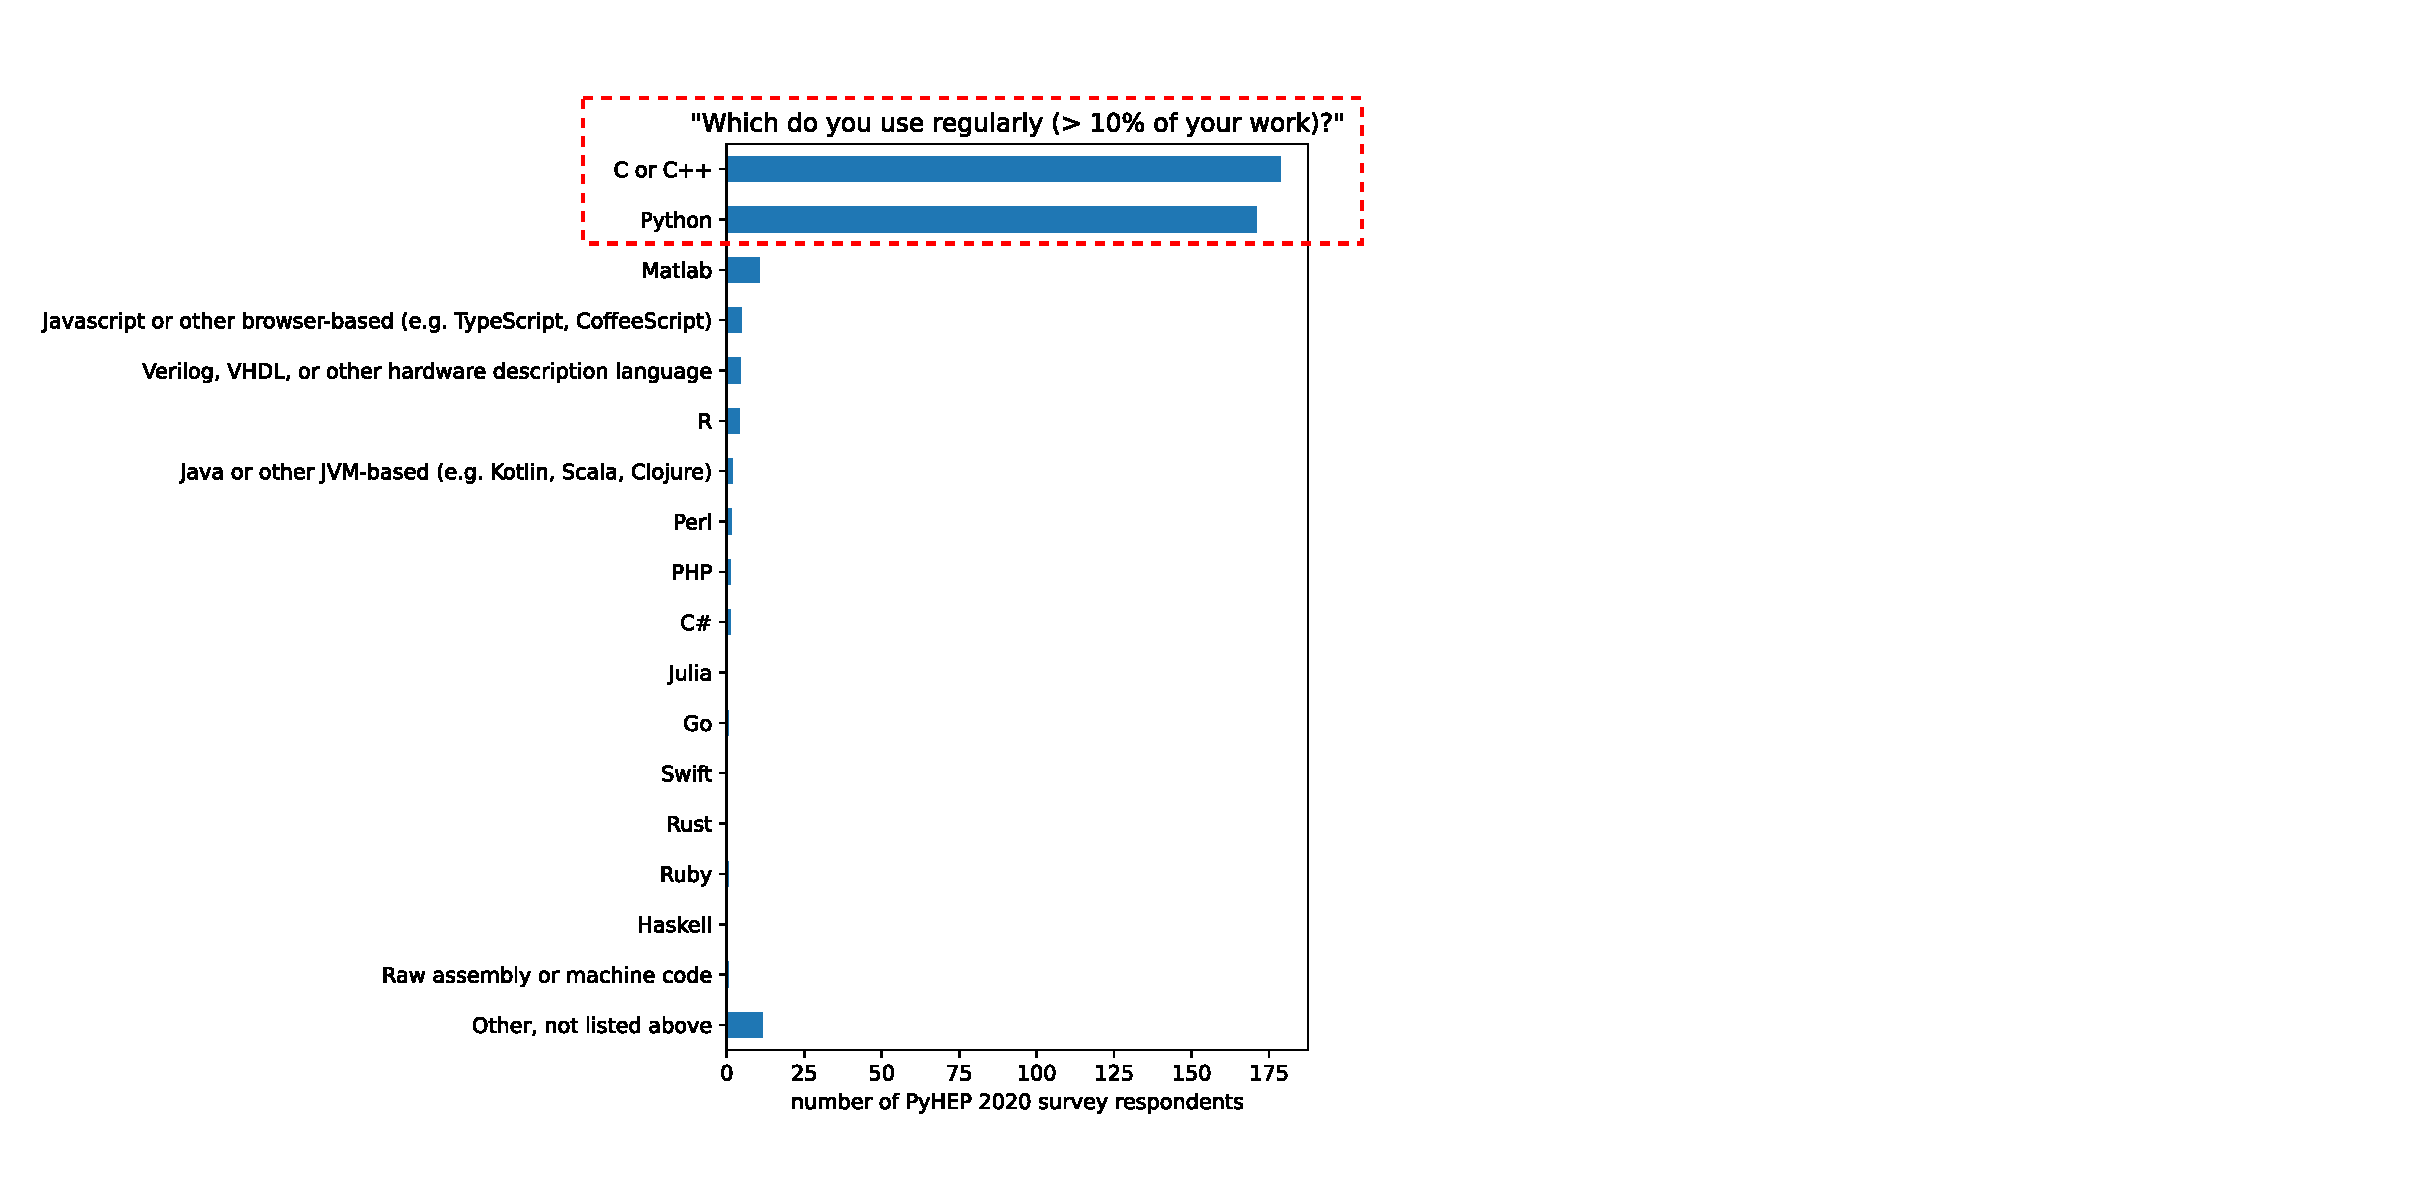
\includegraphics[width=\linewidth]{pyhep2020-survey-2.pdf}}\only<3>{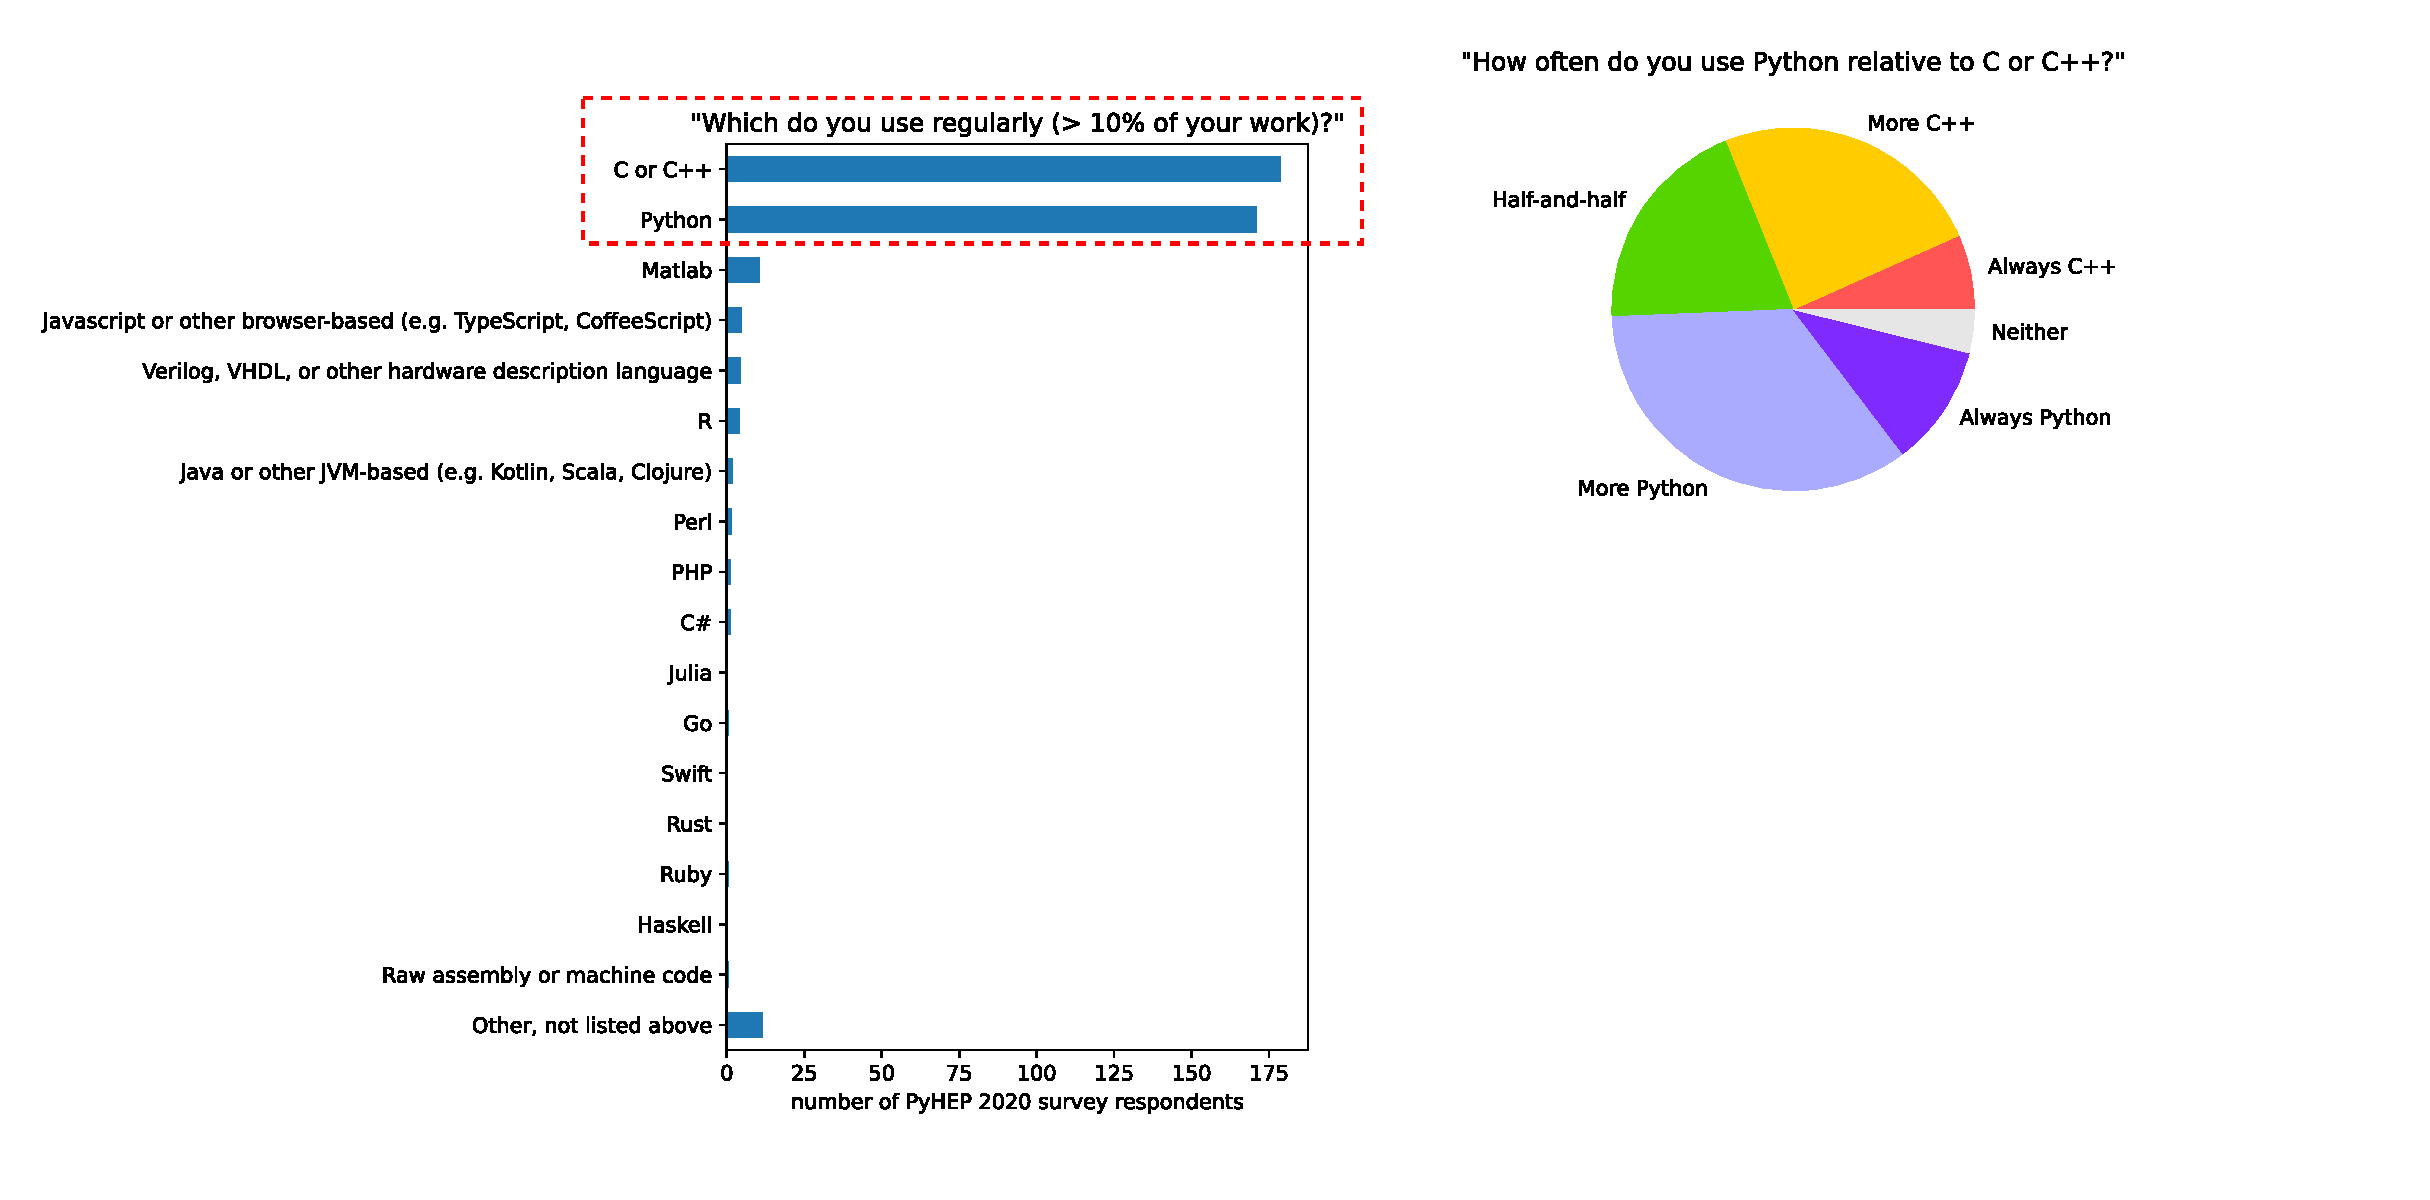
\includegraphics[width=\linewidth]{pyhep2020-survey-3.pdf}}\only<4>{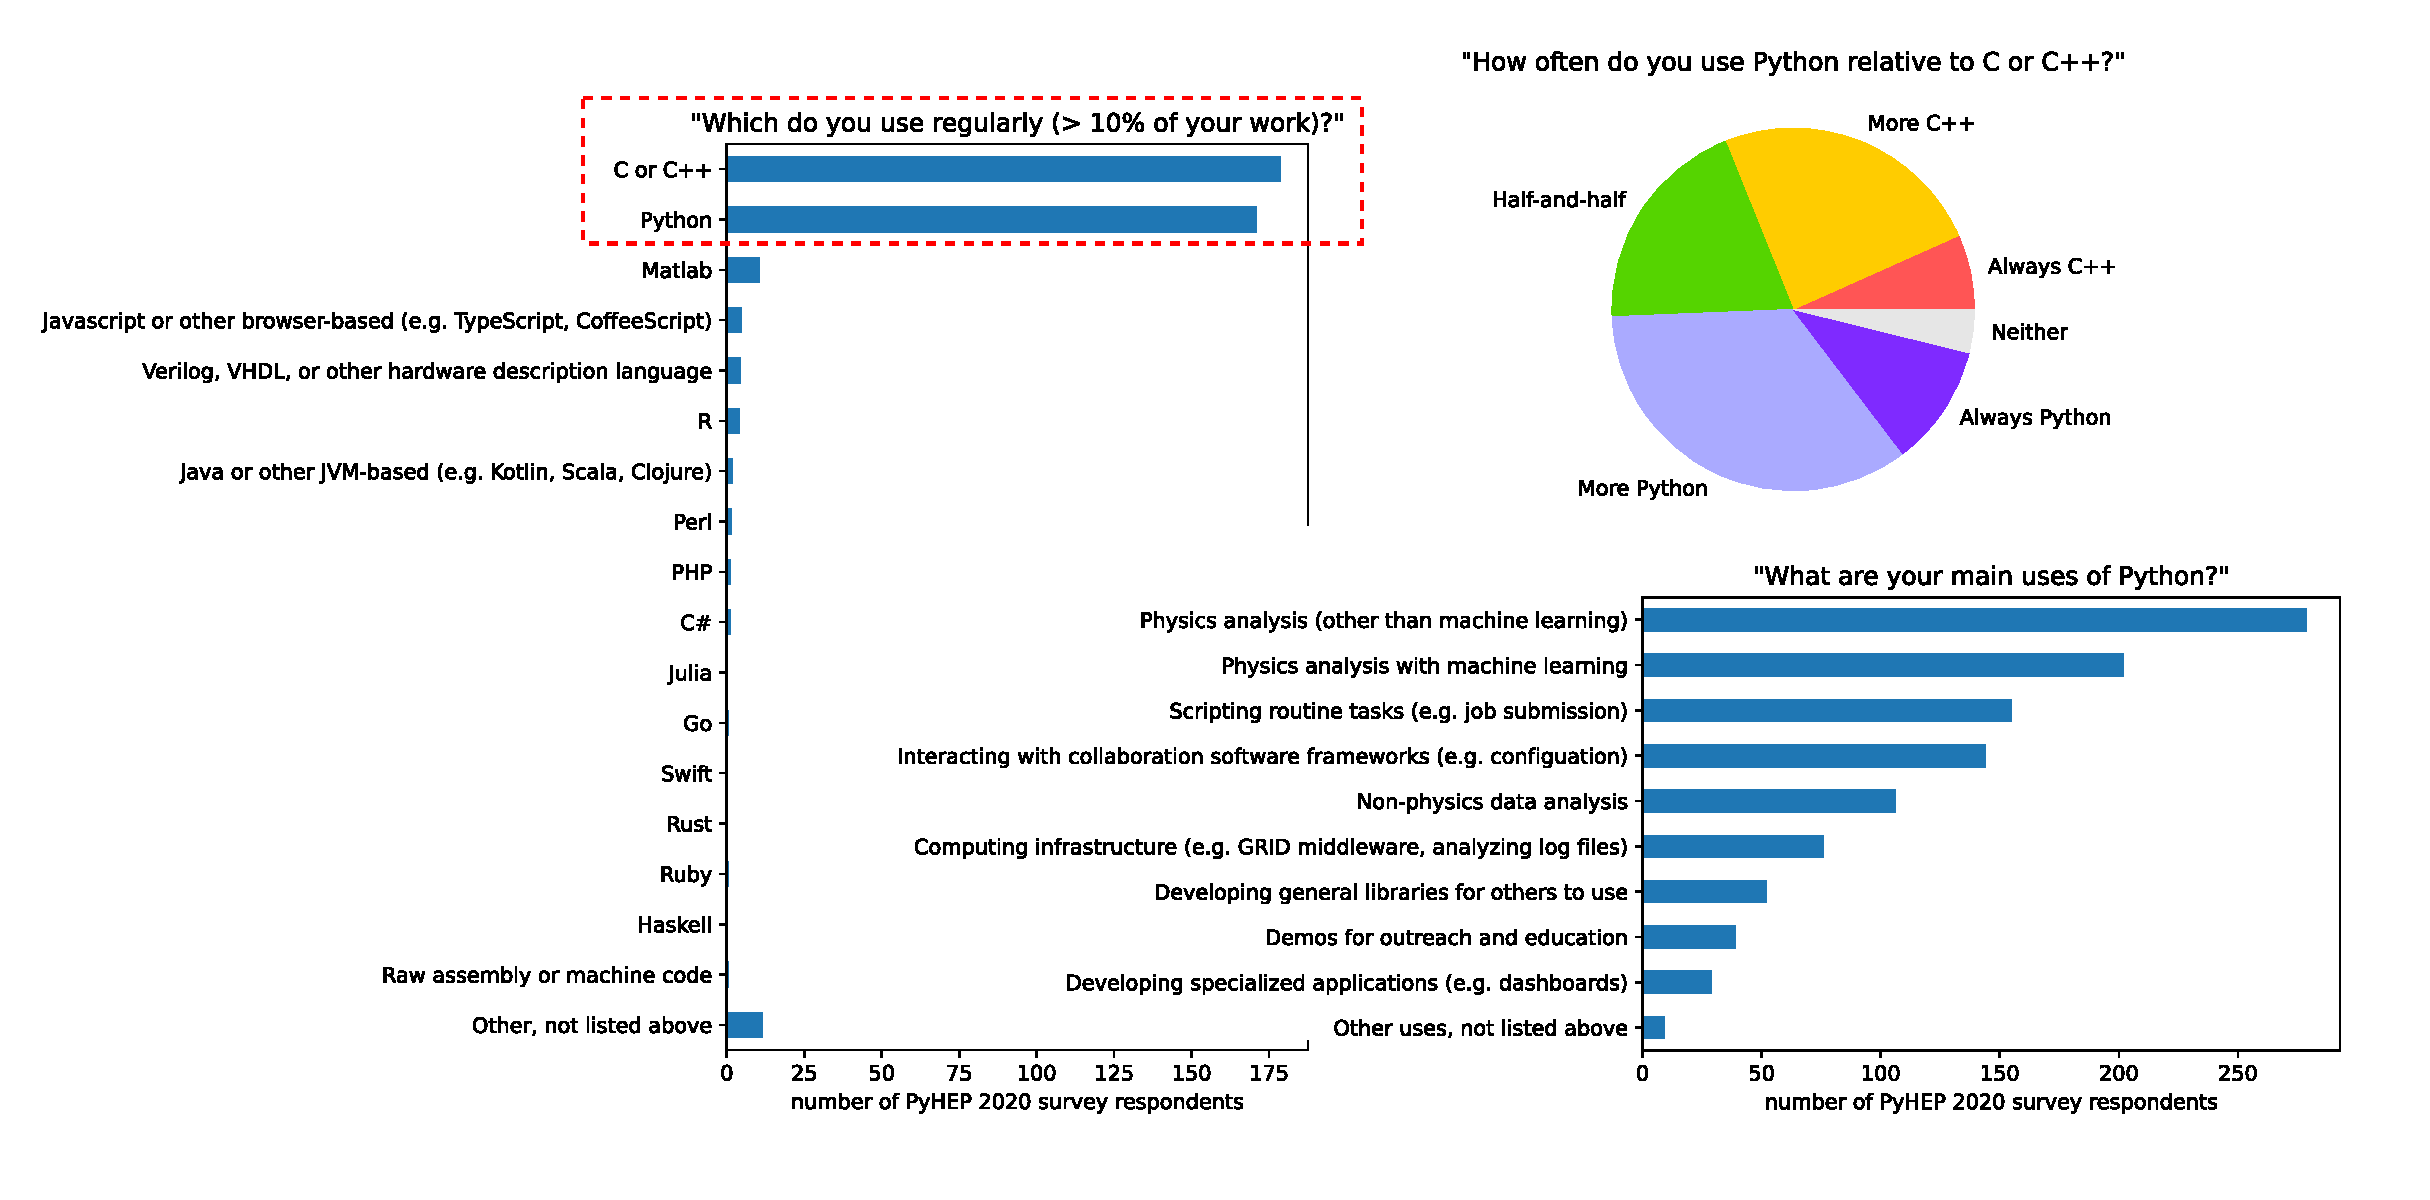
\includegraphics[width=\linewidth]{pyhep2020-survey-4.pdf}}\only<5>{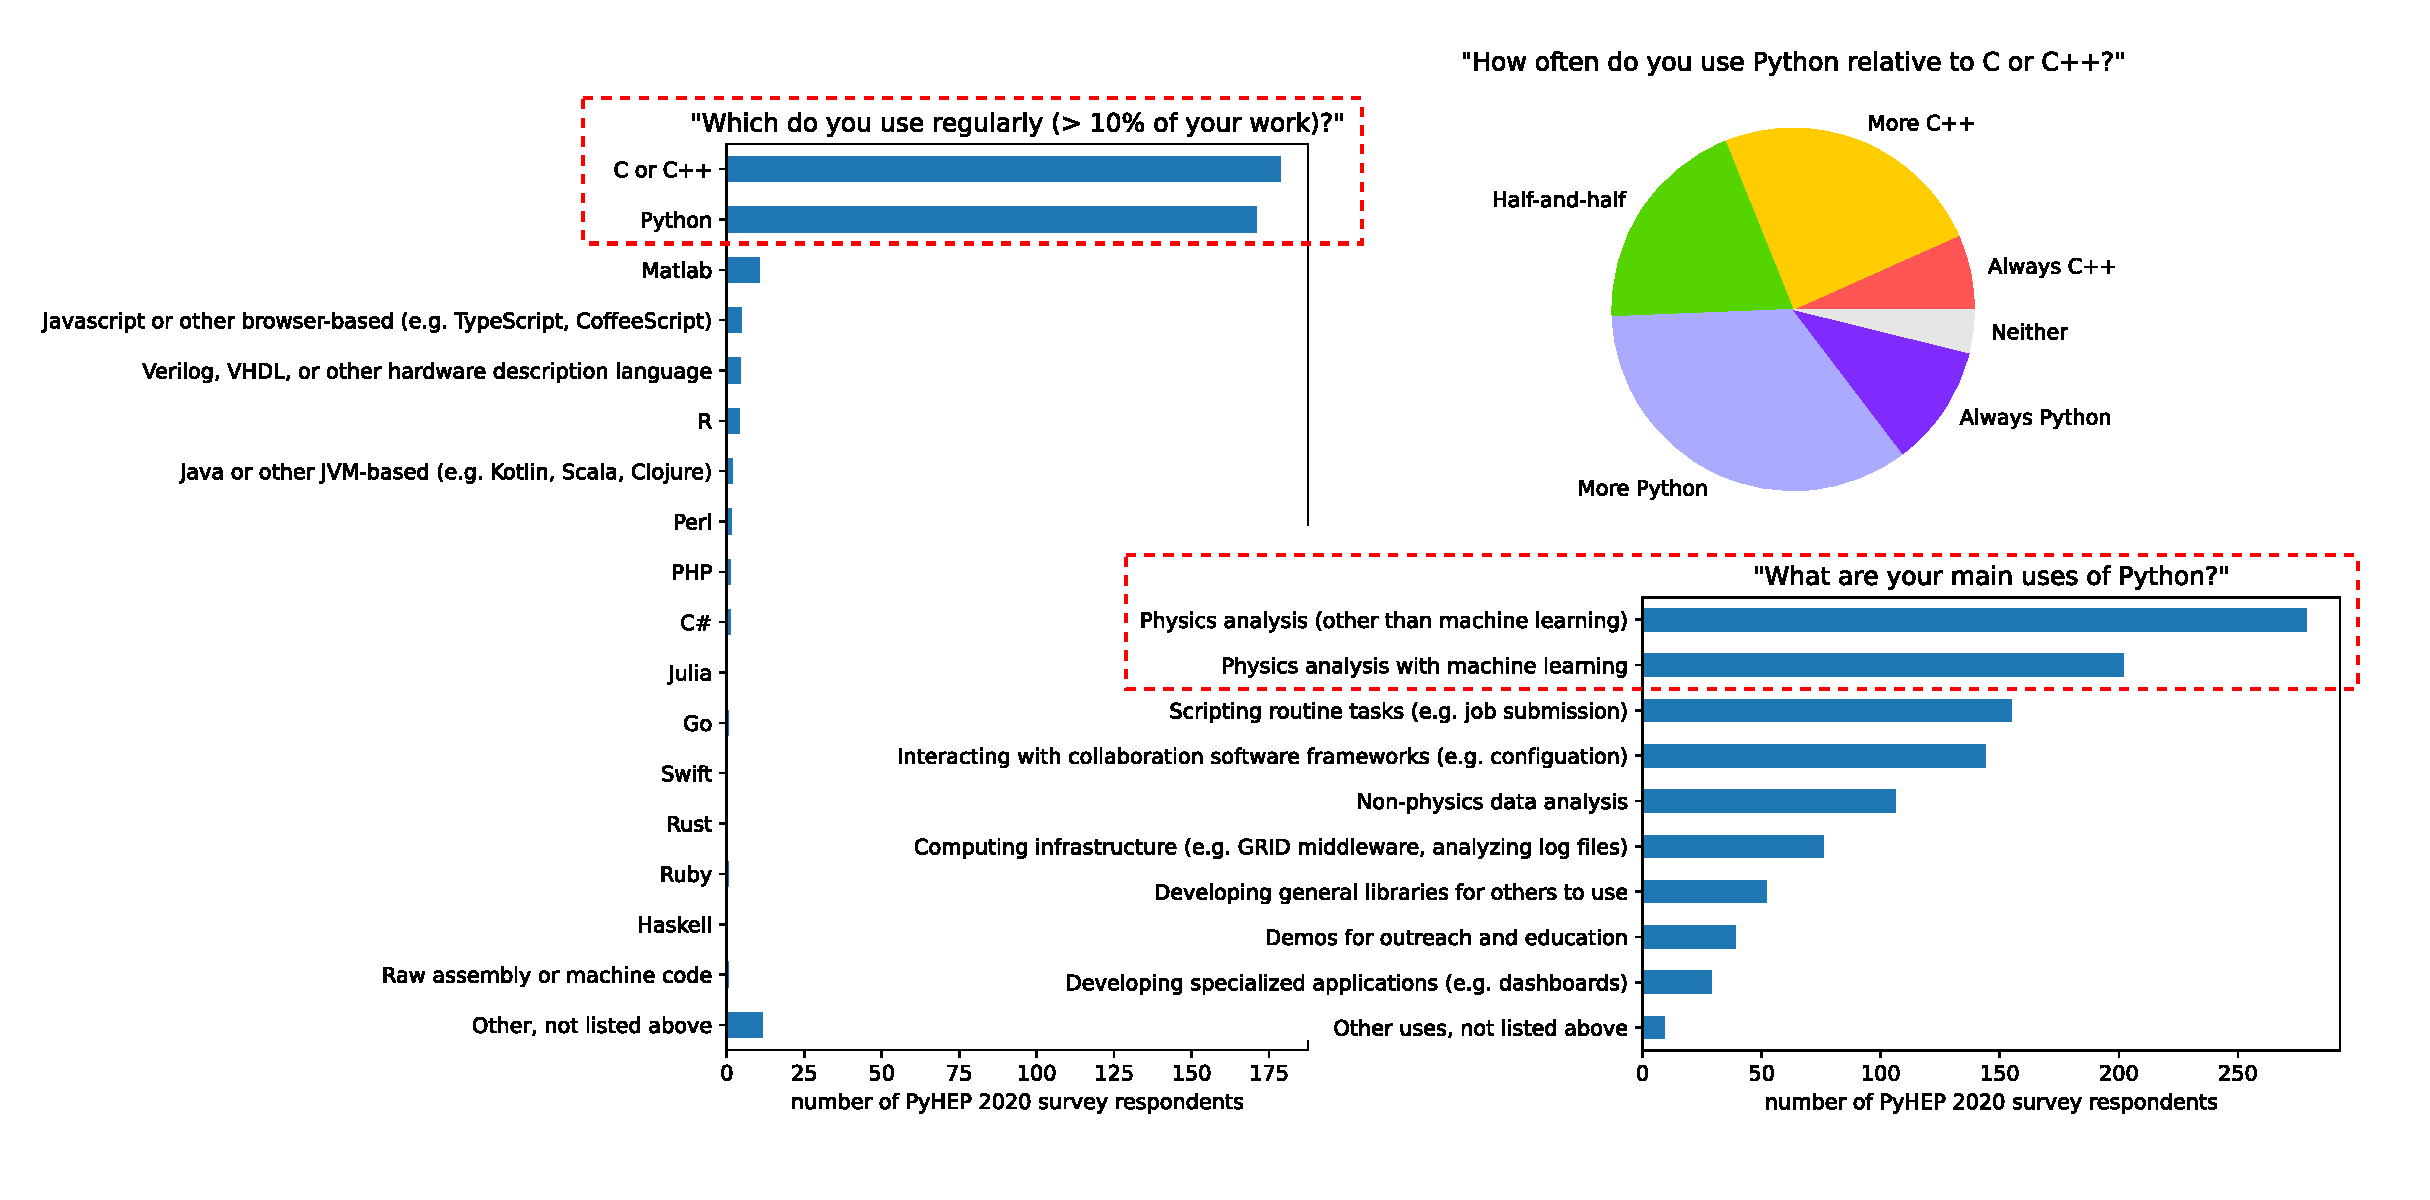
\includegraphics[width=\linewidth]{pyhep2020-survey-5.pdf}}
\end{columns}
\end{frame}

\begin{frame}{This community is also tolerant of significant API changes}
\vspace{0.25 cm}
\textcolor{darkblue}{\mbox{\hspace{-0.5 cm}}PyPI download statistics of \only<1>{Uproot 3 $\to$ 4}\only<2>{Awkward Array 0 $\to$ 1}}

\vspace{-0.03 cm}
\begin{columns}
\column{1.08\linewidth}
\only<1>{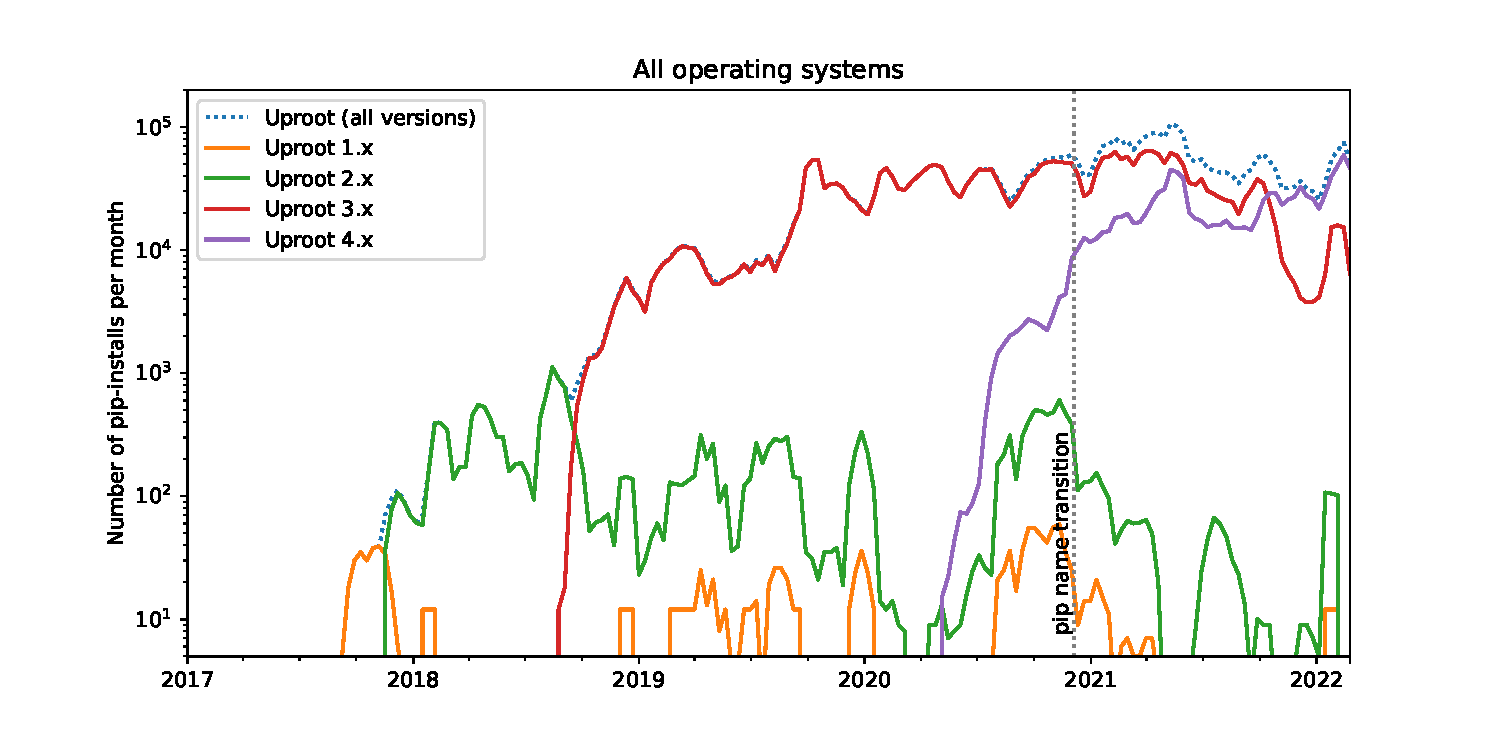
\includegraphics[width=\linewidth]{pip-allos-uproot-log.pdf}}\only<2>{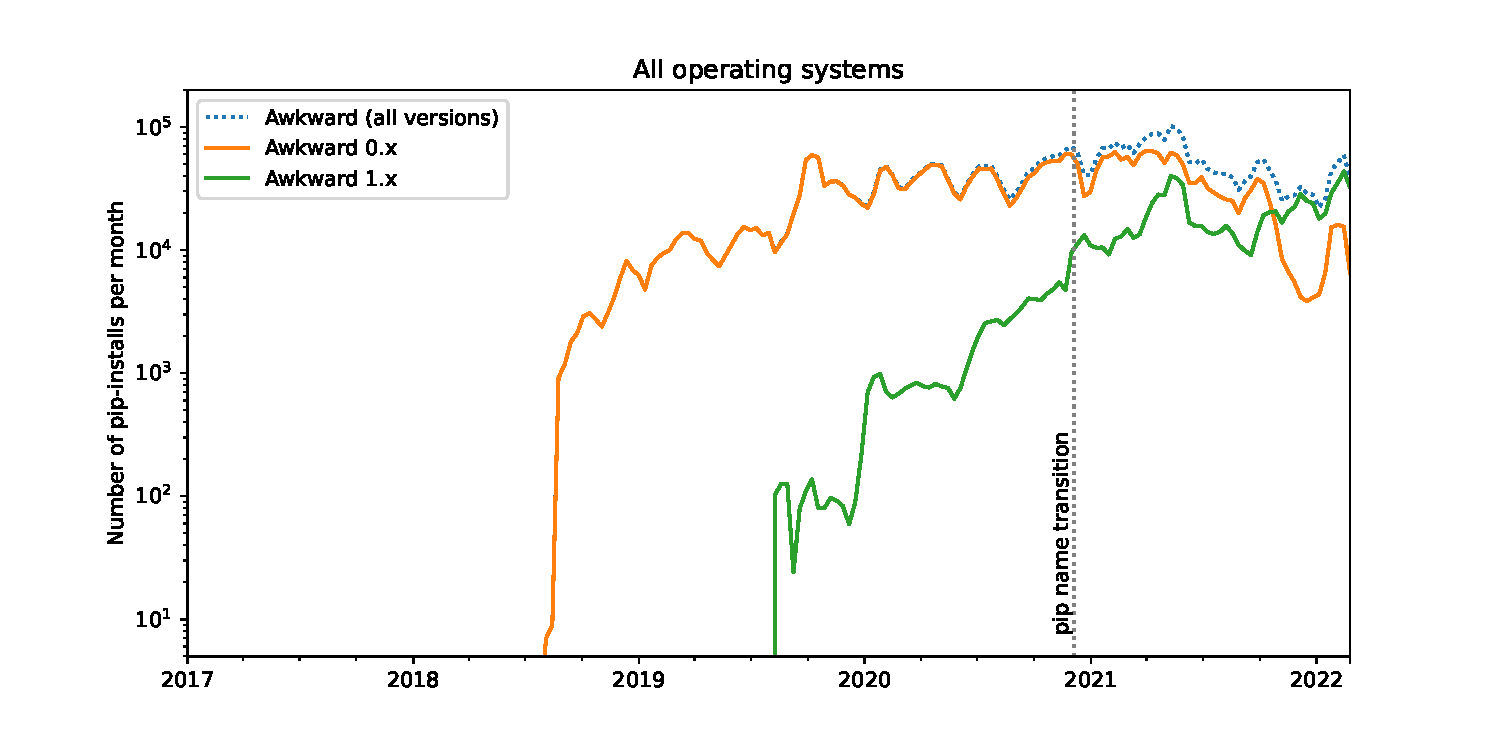
\includegraphics[width=\linewidth]{pip-allos-awkward-log.pdf}}
\end{columns}
\end{frame}

\begin{frame}{And we're seeing interest from outside the HEP community, too}
\vspace{0.25 cm}
\textcolor{darkblue}{\mbox{\hspace{-0.5 cm}}GitHub stars versus time}

\vspace{0.25 cm}
\begin{columns}
\column{0.75\linewidth}
\only<1>{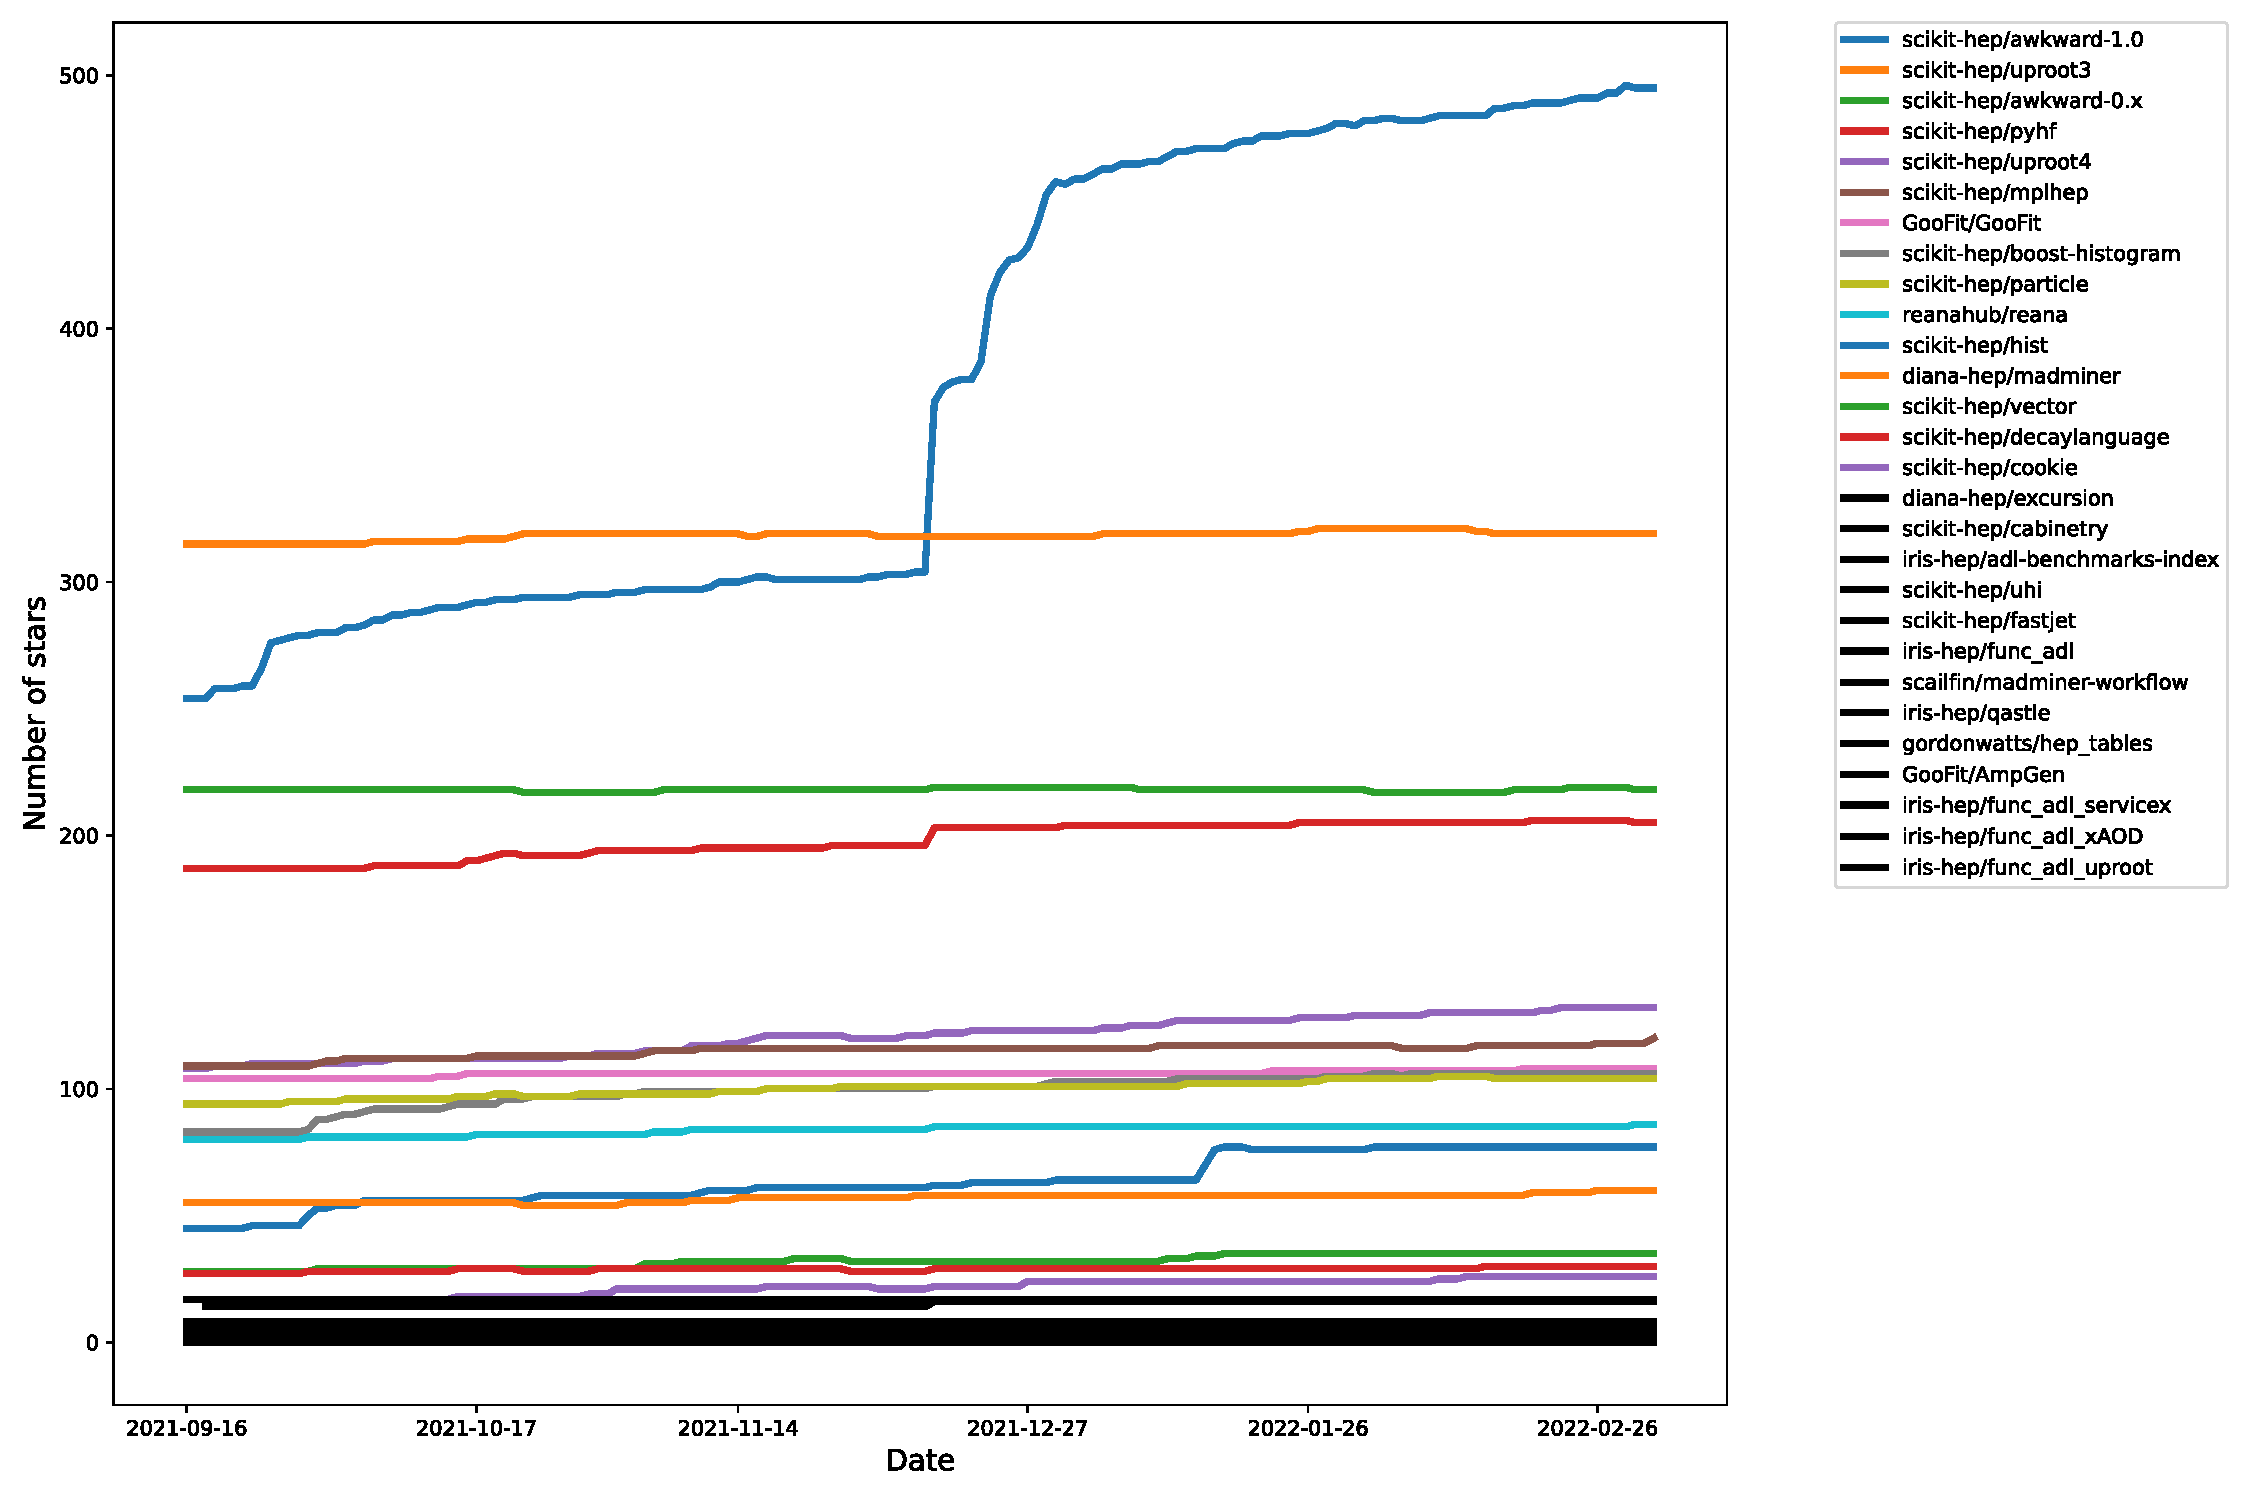
\includegraphics[width=\linewidth]{irishep-as-stars-1.pdf}}\only<2>{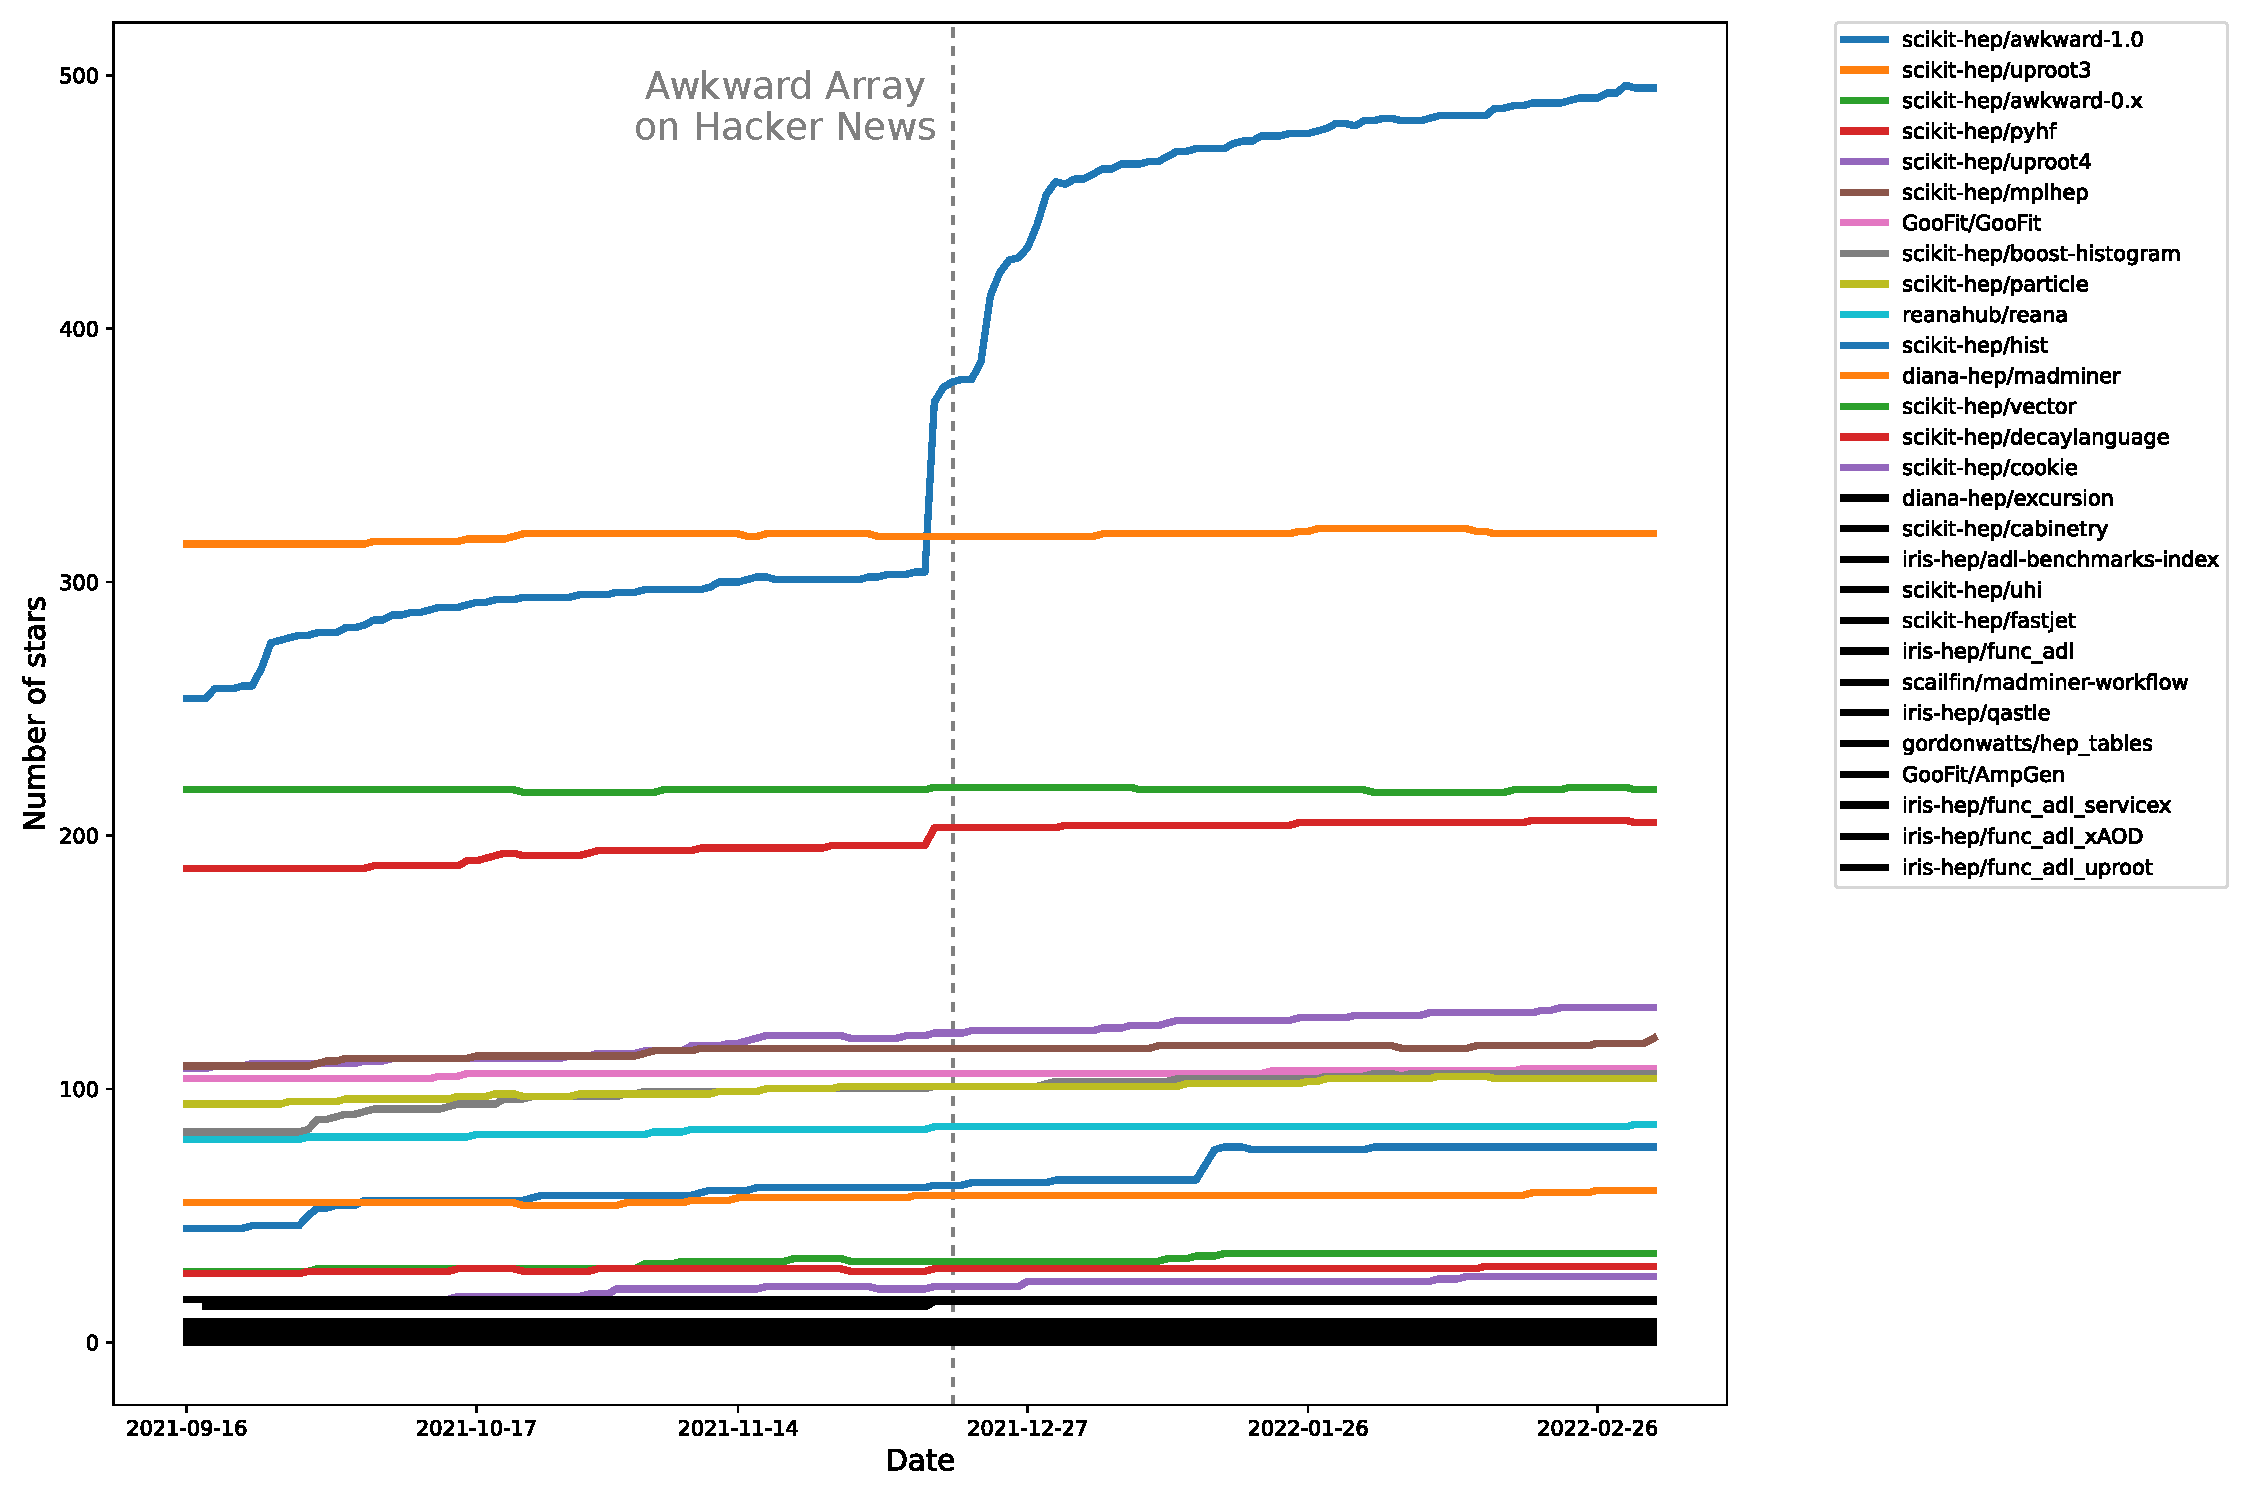
\includegraphics[width=\linewidth]{irishep-as-stars-2.pdf}}

\column{0.25\linewidth}
\uncover<2->{\small\textcolor{blue}{\url{https://news.ycombinator.com/item?id=29576323}}}
\end{columns}
\end{frame}

\end{document}
